\chapter{Crystalline properties of TASE-grown nanowires}
\label{chap:properties}

The critical growth mechanisms and single-facet \hkl{111}\(_B\) growth front stabilisation method were explored and developed in Chapter~\ref{chap:growth}. However, the lack of in-plane \hkl{1 1 1} directions in the \hkl(0 0 1) \acf{soi} wafer on which growth was carried out complicates the analysis of the growth results. The two possible \hkl{1 1 1} facets are tilted and, therefore, yield calculations and contacting of devices become more complex, as the process through which one of the facets is selected for stabilisation is dependent on the shape and orientation of the nucleating crystal on the \acs{si} seed.

CHAPTER OVERVIEW

\section{\texorpdfstring{Fabrication on \acs{si}\hkl(1 1 0) \acs{soi}}{Fabrication on Si(110) SOI}}

The fabrication of templates for nanowires and microstructures on the new \hkl(1 1 0) substrate followed the same underlying methodology (see Appendix~\ref{chap:tase}) implemented on the same tools (see Appendix~\ref{chap:tools}) that was used for the samples in Chapter~\ref{chap:growth}. A series of lithography steps, including both \acf{ebl} and uv lithography; deposition steps, including \acf{ald} and \acf{pecvd}; and etching steps, including \acf{rie}, \acf{icp} etching and \acf{tmah} and \acf{hf} etching were employed to define the structures (seed and growth region) enclose them in the template \acs{sio2}, open the template, and finally etch back the sacrificial \acs{si} to expose the seed surface.

\subsection{Template design considerations}


\begin{figure}
    \centering
    \subcaptionbox{
    \hkl(1 1 0) in-plane crystalline directions.
    \label{subfig:110wafer_directions}
    }{
        \begin{tikzpicture}
            \begin{scope}[scale=0.22]
                \draw (90:11cm) -- (90:13cm);
                \draw[stealth-stealth] (90:12cm) arc [start angle = 90, end angle = -90, radius = 12cm] node[midway, anchor = west]{\qty{180}{\degree}};
                \draw (-90:11cm) -- (-90:13cm);
                \draw (-90:10cm) arc [start angle=270, end angle=358.8, radius=10cm] -- (9.8935cm,-1.065mm) arc [start angle=-135, end angle=-225, radius=1.5mm] -- (9.9987cm,2.13mm) arc [start angle=1.20, end angle=90, radius=10cm];
                \draw[dashed] (90:10cm) arc [start angle=90, end angle=270, radius=10cm];
                \path[decorate,decoration={text along path, text={Repeated by symmetry},text align=center}] (315:11) arc [start angle=315,end angle=45,radius=11];
                \draw[dashed] (90:10cm) -- (0, 0) -- (-90:10cm);
                \draw[-stealth, thick] (0, 0) -- ++ (90:4cm) node[anchor=south east] {\hkl[0 0 1]};
                \draw[-stealth, thick] (0, 0) -- ++ (35.3:4cm) node[anchor=south] {\hkl[-1 1 1]};
                \draw[-stealth, thick] (0, 0) node[anchor=east] {\hkl[1 1 0]} -- ++ (0:4cm) node[anchor=west] {\hkl[-1 1 0]};
                \draw[-stealth, thick] (0, 0) -- ++ (270:4cm) node[anchor=north east] {\hkl[0 0 -1]};
                \draw[-stealth, thick] (0, 0) -- ++ (-35.3:4cm) node[anchor=north] {\hkl[-1 1 -1]};
                \node[mark size=2pt] at (0, 0) {\pgfuseplotmark{diamond*}};
            \end{scope}
        \end{tikzpicture}
    }
    \subcaptionbox{
    \acs{si} seed area before growth.
    \label{subfig:110_etchback}
    }{
        \begin{tikzpicture}
            \filldraw[fill=Si_green] (2cm, 0cm) --  node[midway, anchor= north west] {\acs{si}} (2cm, 22mm) -- (4cm, 22mm) -- (4cm, 0cm) node[midway, anchor=west]{{\hkl{1 1 1}}} -- cycle;
            \filldraw[fill=SiO2_blue] (0cm, -10mm) -- (8cm, -10mm) -- (8cm, 0cm) -- (2cm, 0mm)-- (2cm, 22mm) -- (8cm, 22mm) -- (8cm, 32mm) -- (0cm, 32mm) --  node[midway, anchor=west] {\acs{sio2}} cycle; 
            \draw (3.7cm, 22mm) arc [start angle = 180, end angle = 270, radius = 3mm] node[midway, anchor = north east]{\qty{90}{\degree}};
            \draw[-stealth] (6cm, 7mm) node[anchor=north] {\hkl<-1 1 -2>} -- ++ (90:0.8cm) node[anchor=south] {\hkl<1 1 0>};
            \draw[-stealth] (6cm, 7mm) -- ++ (0:0.8cm) node[anchor=west] {\hkl<-1 1 1>};
            \node[mark size=2pt] at (6, 7mm) {\pgfuseplotmark{o}};
        \end{tikzpicture}
    }
    \caption{Crystalline orientations in the \hkl[1 1 0] \acs{soi} wafer. \subref{subfig:110wafer_directions} shows a schematic of the crystalline directions in the plane of the \acs{si} device layer, highlighting its two-fold symmetry. \subref{subfig:110_etchback} highlights the high-symmetry directions in the \hkl{1 1 2} plane containing the chosen \hkl<1 1 1> growth direction and the \hkl[1 1 0] vector defining the wafer orientation. It highlights the vertical \hkl{1 1 1} seed facet.}
    \label{fig:110_wafer_properties}
\end{figure}

An initial evaluation of the crystalline symmetry in the wafer plane is necessary to plan the orientation of the \acf{tase} templates on the wafer surface. Figure~\ref{subfig:110wafer_directions} shows the various in-plane crystalline directions in the top device layer of the \hkl(1 1 0) \acs{soi} wafer employed in the fabrication of all future samples. Unlike its \hkl(001) predecessor, which had a four-fold axis perpendicular to the wafer plane, this \hkl(1 1 0) wafer has a two-fold axis dictating the in-plane symmetry. Therefore, the wafer's notch becomes key to orienting the \acs{tase} structures with the desired crystalline directions.
\par
Figure~\ref{subfig:110_etchback} shows a schematic cross-section of the \acs{tase} structure before growth with colour-coded materials. The \acs{si} seed presents a \hkl{1 1 1} facet forming a \qty{90}{\degree} angle with all the template walls because of the \acs{tmah} etchant used to remove the sacrificial \acl{si}; unlike the \hkl<0 0 1> wafer samples which formed \qty{90}{\degree} angles with the sidewalls (Figure~\ref{subfig:enterprise_etchback}).

\begin{sidewaysfigure}
    \centering
    \subcaptionbox{
    Double comb structure evolution from the comb structure in Figure~\ref{subfig:enterprise_design}.
    \label{subfig:110_design1}
    }{
        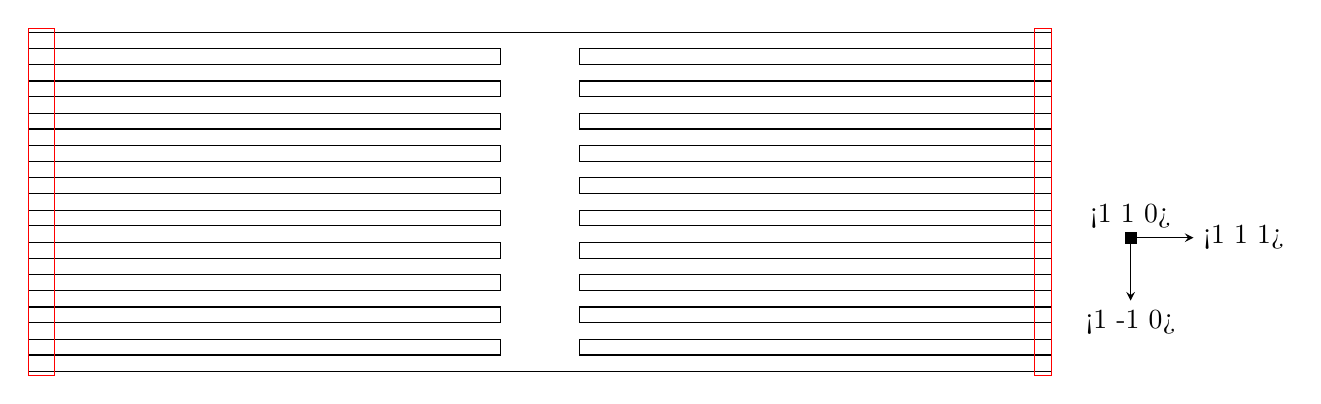
\begin{tikzpicture}
            \begin{scope}[]
                \draw (0, 0) -- ++ (13, 0) -- ++ (0, 0.21) -- ++ (-6, 0) -- ++ (0, 0.2) -- ++ (6, 0) -- ++ (0, 0.21) -- ++ (-6, 0) -- ++ (0, 0.2) -- ++ (6, 0) -- ++ (0, 0.21) -- ++ (-6, 0) -- ++ (0, 0.2) -- ++ (6, 0) -- ++ (0, 0.21) -- ++ (-6, 0) -- ++ (0, 0.2) -- ++ (6, 0) -- ++ (0, 0.21) -- ++ (-6, 0) -- ++ (0, 0.2) -- ++ (6, 0) -- ++ (0, 0.21) -- ++ (-6, 0) -- ++ (0, 0.2) -- ++ (6, 0) -- ++ (0, 0.21) -- ++ (-6, 0) -- ++ (0, 0.2) -- ++ (6, 0) -- ++ (0, 0.21) -- ++ (-6, 0) -- ++ (0, 0.2) -- ++ (6, 0) -- ++ (0, 0.21) -- ++ (-6, 0) -- ++ (0, 0.2) -- ++ (6, 0) -- ++ (0, 0.21) -- ++ (-6, 0) -- ++ (0, 0.2) -- ++ (6, 0) -- ++ (0, 0.21) -- ++ (-13, 0) -- ++ (0, -0.21) -- ++ (6, 0) -- ++ (0, -0.2) -- ++ (-6, 0) -- ++ (0, -0.21) -- ++ (6, 0) -- ++ (0, -0.2) -- ++ (-6, 0) -- ++ (0, -0.21) -- ++ (6, 0) -- ++ (0, -0.2) -- ++ (-6, 0) -- ++ (0, -0.21) -- ++ (6, 0) -- ++ (0, -0.2) -- ++ (-6, 0) -- ++ (0, -0.21) -- ++ (6, 0) -- ++ (0, -0.2) -- ++ (-6, 0) -- ++ (0, -0.21) -- ++ (6, 0) -- ++ (0, -0.2) -- ++ (-6, 0) -- ++ (0, -0.21) -- ++ (6, 0) -- ++ (0, -0.2) -- ++ (-6, 0) -- ++ (0, -0.21) -- ++ (6, 0) -- ++ (0, -0.2) -- ++ (-6, 0) -- ++ (0, -0.21) -- ++ (6, 0) -- ++ (0, -0.2) -- ++ (-6, 0) -- ++ (0, -0.21) -- ++ (6, 0) -- ++ (0, -0.2) -- ++ (-6, 0) -- ++ (0, -0.21);
                \draw[red] (0, -0.05) rectangle (0.333, 4.36);
                \draw[red] (12.777, -0.05) rectangle (13, 4.36);
            \end{scope}
            \begin{scope}[shift={(14cm, 1.7cm)}]
                \draw[-stealth] (0cm, 0cm) -- ++ (-90:0.8cm) node[anchor=north] {\hkl<1 -1 0>};
                \draw[-stealth] (0cm, 0cm)  node[anchor=south] {\hkl<1 1 0>} -- ++ (0:0.8cm) node[anchor=west] {\hkl<1 1 1>};
                \node[mark size=2pt] at (0, 0) {\pgfuseplotmark{square*}};
            \end{scope}
        \end{tikzpicture}
    }
    \subcaptionbox{
    Array structure evolved from the double comb structure of \subref{subfig:110_design1} and merge wire structure on the bottom right.
    \label{subfig:110_design2}
    }{
        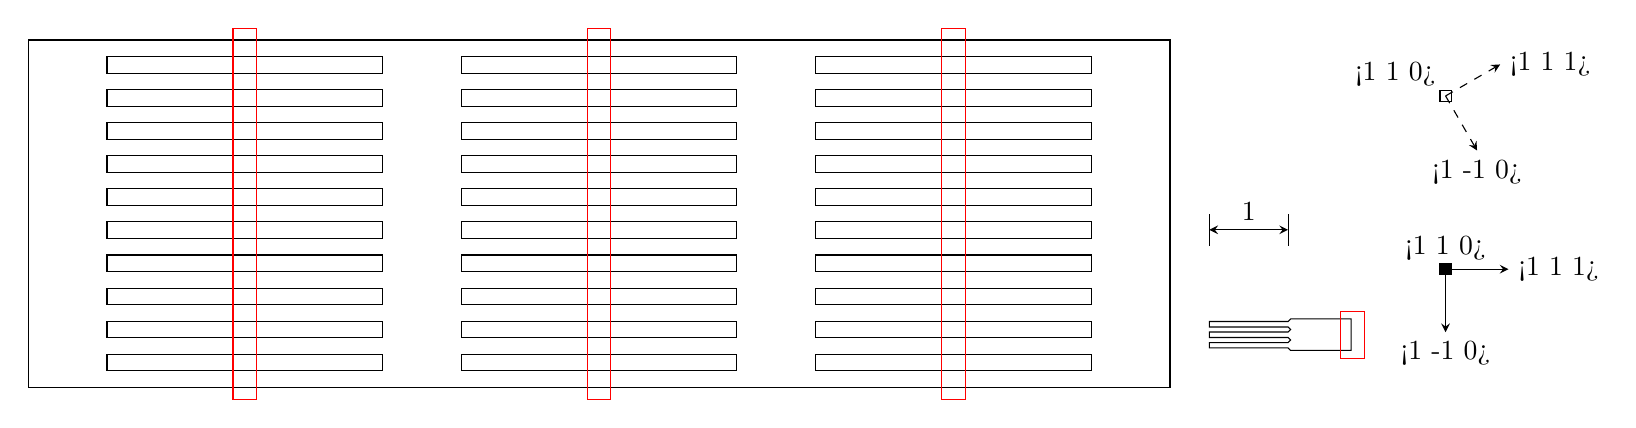
\begin{tikzpicture}
            \begin{scope}
                \draw (0, 0) rectangle (14.5, 4.41);
                \foreach \x in {1, 5.5, 10}
                    \foreach \y in {1, 3, 5, 7, 9, 11, 13, 15, 17, 19}
                        \draw (\x, \y*0.21) rectangle (\x+3.5, 0.21+\y*0.21);
                \foreach \x in {2.6, 7.1, 11.6}
                    \draw [red] (\x, -0.15) rectangle (\x+0.3, 4.56);
            \end{scope}
            \begin{scope}[shift={(15cm, 0.5cm)}]
                \draw (0,0) -- ++ (1, 0) -- ++ (-45:0.045255) -- ++ (0.768, 0) -- ++ (0, 0.4) -- ++ (-0.768, 0) -- ++ (-135:0.045255) -- ++ (-1, 0) -- ++ (0, -0.07) -- ++ (1, 0) -- ++ (-45:0.045255) -- ++ (-135:0.045255) -- ++ (-1, 0) -- ++ (0, -0.07) -- ++ (1, 0) -- ++ (-45:0.045255) -- ++ (-135:0.045255) -- ++ (-1, 0) -- cycle;
                \draw [red] (1.668, -0.132) rectangle (1.968, 0.468);
                \draw[stealth-stealth] (0, 1.5) -- (1, 1.5) node [midway, anchor = south] {\qty{1}{\micro\metre}};
                \draw (0, 1.3) -- (0, 1.7);
                \draw (1, 1.3) -- (1, 1.7);
            \end{scope}
            \begin{scope}[shift={(18cm, 1.5cm)}]
                \draw[-stealth] (0cm, 0cm) -- ++ (-90:0.8cm) node[anchor=north] {\hkl<1 -1 0>};
                \draw[-stealth] (0cm, 0cm)  node[anchor=south] {\hkl<1 1 0>} -- ++ (0:0.8cm) node[anchor=west] {\hkl<1 1 1>};
                \node[mark size=2pt] at (0, 0) {\pgfuseplotmark{square*}};
            \end{scope}
            \begin{scope}[shift={(18cm, 3.7cm)}, rotate=30]
                \draw[-stealth, dashed] (0cm, 0cm) -- ++ (-90:0.8cm) node[anchor=north] {\hkl<1 -1 0>};
                \draw[-stealth, dashed] (0cm, 0cm)  node[anchor=south east] {\hkl<1 1 0>} -- ++ (0:0.8cm) node[anchor=west] {\hkl<1 1 1>};
                \node[mark size=2pt] at (0, 0) {\pgfuseplotmark{square}};
            \end{scope}
        \end{tikzpicture}
    }
    \caption{Microstructure designs for \acs{tase} growth. The structures transferred to the \acs{si} device layer are represented in black and the template opening regions in red. \subref{subfig:110_design1} shows the double comb structures grown on the first \hkl[1 1 0] samples. These were always oriented to have the template axis coincide with the in-plane \hkl<1 1 1> directions. \subref{subfig:110_design2} shows the nanowire array structures used in later experiments on the \hkl[1 1 0] \acs{soi}s and the "merge wire" structures. These types of structures were grown both aligned with the in-plane \hkl[1 1 1] direction, as highlighted by the solid-line arrows, and \qty{30}{\degree} misaligned, as shown by the dashed arrows \cite{Brugnolotto2023_2}.}
    \label{fig:110_Template_Design}
\end{sidewaysfigure}

Figure~\ref{fig:110_Template_Design} shows the evolution of the \acs{tase} structures from those in Figure~\ref{fig:001_Templat5e_Design}. The comb structure of Figure~\ref{subfig:enterprise_design} is perfect for \acf{sem_m} analysis of multiple wires in a single image and the \acf{stem_m} survey of cross-section cuts perpendicular to the growth direction. However, cross-sections parallel to the growth direction only allow for the analysis of a single wire.
\par
As the analysis of heterointerfaces stacked along the growth vector is the primary goal of this work, maximising the number of wires observable from seed to final interface in a single \acf{fib} cut is a key objective of the design phase. Taking inspiration from the "T-shaped" structure in Figure~\ref{subfig:enterprise_design} the first evolution of the comb array is shown in Figure~\ref{subfig:110_design1}. A central rectangular \acs{si} backbone anchors two rows of nanowires that extend from either side, with the templates being open at the very edges of the structure (in red in Figure~\ref{subfig:110_design1}. The length of the nanowire growth area extends up to \qty{7}{\micro\metre} for this design. These long channels (in relation to their \qty{70}{\nano\metre} height) were designed to study the effect of growth in "deep" templates on resulting composition and growth rates. Unfortunately, in practice, the resulting structure could only be used with short etch-back segments. This was due to the thickness of the side walls in the final samples, which was insufficient to ensure structural integrity during \acs{tmah} etch-back, despite the selectivity of this etchant.
\par
The difficulties encountered with the design in Figure~\ref{subfig:110_design1} together with the possibility of having more \acs{stem_m}-observable nanowires per \acs{fib} cut led to the design of the array structure in Figure~\ref{subfig:110_design2}. This allows for the \acs{stem_m} analysis of \num{6} short nanowires up to \qty{2}{\micro\metre}-long while keeping the overall length of the structure at \qty{14.5}{\micro\metre}, and therefore comparable to that of the double-comb design (\qty{13}{\micro\metre}). There are \num{4} equidistant rectangular backbone anchors, with two marking the beginning and end of the structure. The templates are open between the anchors in three areas of the structures (in red in Figure~\ref{subfig:110_design2}). Thus, once complete, one such array contains \num{66} growth sites.

Wire widths of \qty{70}{\nano\metre}, \qty{140}{\nano\metre}, \qty{210}{\nano\metre}, and \qty{280}{\nano\metre} were fabricated, the Figures~\ref{subfig:110_design1} and \ref{subfig:110_design2} show the \qty{210}{\nano\metre} designs.

To the bottom right of the array in Figure~\ref{subfig:110_design2} there is a "merge wire" structure. In this structure, three nucleation wires with a design width of \qty{70}{\nano\metre} all terminate in a single channel \qty{400}{\nano\metre} wide. This structure was designed to study the merging regions between the three growing crystals to observe the defects that could form from the merging of two growing crystals. In the past, it was employed to demonstrate the introduction of dislocations in \acs{tase} microstructures \cite{Mauthe2021} and published research highlighted the formation of defects at those sites due to minuscule misalignments of the crystals \cite{Jacobsson2015, Rossi2023}.

Both structures in Figure~\ref{subfig:110_design2} were grown aligned to the in-plane \hkl<1 1 1> direction but also \qty{30}{\degree} misaligned. In practice, this was done by aligning one set of structures to an in-plane \hkl<1 1 1> direction and rotating each subsequent set by \qty{90}{\degree}. Selecting this specific \qty{30}{\degree} misalignment as a basis for analysis therefore has two advantages:
\begin{enumerate}
    \item the resulting seed surfaces and projected growth fronts are at a significant angle with the template sidewalls
    \item there is no need to keep track of the direction of the notch past the dicing stage which resulted in the initial \qtyproduct{6 x 6}{cm} die.
\end{enumerate}

\subsection{\texorpdfstring{\acs{fib} lamella fabrication}{FIB lamella fabrication}}

\begin{figure}
    \centering
    \begin{tikzpicture}[isometric]
        \draw (0, 0, 0) -- (0, 0, 2) -- (0, 1, 2) -- (0, 1, 0) -- cycle;
        \draw (0, 0, 0) -- (3, 0, 0) -- (3, 1, 0) -- (0, 1, 0);
        \draw (0, 0, 2) -- (3, 0, 2) -- (3, 1, 2) -- (0, 1, 2);
        \draw (3, 0, 0) -- (3, 0, 2);
        \draw (3, 1, 0) -- (3, 1, 2);
            
        \draw (-0.2, 0, -0.2) -- (-0.2, 0, 2.2) -- (-0.2, 1.2, 2.2) -- (-0.2, 1.2, -0.2) -- cycle;
        \draw (-0.2, 0, -0.2) -- (5, 0, -0.2) -- (5, 1.2, -0.2) -- (-0.2, 1.2, -0.2);
        \draw (-0.2, 0, 2.2) -- (5, 0, 2.2) -- (5, 1.2, 2.2) -- (-0.2, 1.2, 2.2);
        \draw (5, 0, -0.2) -- (5, 0, 2.2);
        \draw (5, 1.2, -0.2) -- (5, 1.2, 2.2);
            
        \path [fill=red!50!, fill opacity=0.3] (-0.5, 0.2, -0.5) -- (-0.5, 0.2, 2.5) -- (5.5, 0.2, 2.5) -- (5.5, 0.2, -0.5) -- cycle;
        \path [fill=red!50!, fill opacity=0.3] (-0.5, 0.8, -0.5) -- (-0.5, 0.8, 2.5) -- (5.5, 0.8, 2.5) -- (5.5, 0.8, -0.5) -- cycle;
            
        \draw [red, dashed] (-0.2, 0.2, -0.2) -- (5, 0.2, -0.2) -- (5, 0.2, 2.2) -- (-0.2, 0.2, 2.2) -- cycle;
        \draw [red, dashed] (-0.2, 0.8, -0.2) -- (5, 0.8, -0.2) -- (5, 0.8, 2.2) -- (-0.2, 0.8, 2.2) -- cycle;

        \begin{scope}[shift={(6, 6, 1)}]
            \draw [-stealth] (0, 0, 0) -- ++ (1, 0, 0) node[anchor = north west]{\hkl<-1 1 1>};
            \draw [-stealth] (0, 0, 0) -- ++ (0, 1, 0) node[anchor = south]{\hkl<1 1 0>};
            \draw [-stealth] (0, 0, 0) -- ++ (0, 0.5, 0.866) node[anchor = east]{\hkl<0 1 -1>};
            \draw [-stealth] (0, 0, 0) -- ++ (0, 0.5, -0.866) node[anchor = south west]{\hkl<1 0 1>};
            \draw [-stealth] (0, 0, 0) -- ++ (0, 0, 1) node[anchor = north east]{\hkl<-1 1 -2>};
        \end{scope}

        \begin{scope}[shift={(10, 5, 0)}]
            \draw (0, 0, 0) -- (0, 0, 2) -- (0, 1, 2) -- (0, 1, 0) -- cycle;
            \draw (0, 0, 0) -- (3, 0, 0) -- (3, 1, 0) -- (0, 1, 0);
            \draw (0, 0, 2) -- (3, 0, 2) -- (3, 1, 2) -- (0, 1, 2);
            \draw (3, 0, 0) -- (3, 0, 2);
            \draw (3, 1, 0) -- (3, 1, 2);
            
            \draw (-0.2, 0, -0.2) -- (-0.2, 0, 2.2) -- (-0.2, 1.2, 2.2) -- (-0.2, 1.2, -0.2) -- cycle;
            \draw (-0.2, 0, -0.2) -- (5, 0, -0.2) -- (5, 1.2, -0.2) -- (-0.2, 1.2, -0.2);
            \draw (-0.2, 0, 2.2) -- (5, 0, 2.2) -- (5, 1.2, 2.2) -- (-0.2, 1.2, 2.2);
            \draw (5, 0, -0.2) -- (5, 0, 2.2);
            \draw (5, 1.2, -0.2) -- (5, 1.2, 2.2);

            \path [fill=red!50!, fill opacity=0.3] (-0.54641016, -0.3, 0.22679492) -- (-0.54641016, 1.5, 1.2660254) -- (5.57735027, 1.5, 1.2660254) -- (5.57735027, -0.3, 0.22679492) -- cycle;
            \path [fill=red!50!, fill opacity=0.3] (-0.54641016, -0.3, 1.12679492) -- (-0.54641016, 1.5, 2.1660254) -- (5.57735027, 1.5, 2.1660254) -- (5.57735027, -0.3, 1.12679492) -- cycle;
        
            \draw [red, dashed] (-0.2, 0, 0.4) -- (5, 0, 0.4) -- (5, 1.2, 1.09282032) -- (-0.2, 1.2, 1.09282032) -- cycle;
            \draw [red, dashed] (-0.2, 0, 1.3) -- (5, 0, 1.3) -- (5, 1.2, 1.99282032) -- (-0.2, 1.2, 1.99282032) -- cycle;
        \end{scope}
    \end{tikzpicture}
    \caption{\acs{fib} cutting strategies to expose \hkl{1 1 0} facets from a \hkl[1 1 0]-oriented substrate. The red-shaded planes show how the cut planes are selected to expose the sides of the wire in correspondence to \hkl{1 1 0} facets if the template axis coincides with a \hkl<1 1 1> direction.}
    \label{fig:110_FIB}
\end{figure}

While a new \hkl<1 1 0> wafer and \hkl<1 1 1> template orientation were used for fabrication, the preference for an exposed \hkl{1 1 0} facet for structural analysis with \acs{stem_m} remains unaltered due to this facet allowing easy recognition of a wide variety of crystalline defects \cite{Dasilva2017}. However, the first difficulty is that, as highlighted in Figure~\ref{subfig:110_etchback}, the in-plane crystalline direction perpendicular to the \hkl<1 1 1> template axis is a \hkl<1 1 2>, making the simple cross-section cut used in the previous chapter (Figure~\ref{subfig:FIB_cut_strategy}) unsuitable.

The most obvious \hkl<1 1 0> direction perpendicular to the \hkl<1 1 1> template axis is the one that defines the wafer orientation itself. As shown on the left of Figure~\ref{fig:110_FIB}, a plane-view cut would satisfy orientation requirements and allow for precise \acf{eds} composition maps and an excellent overview of the evolution of the growth front. However, such a cut is much more complex and time-consuming than a cross-sectional cut. The amount of lamella that must be thinned to sub \qty{100}{\nano\metre} thickness to ensure electron transparency increased from a few hundred nanometres to \qty{1.5}{\micro\metre}, which is challenging to do with the ion beam of the \acs{fib} and requires a high level of precision. This is particularly true when milling both sides of a target region composed of multiple material layers eroded at different rates.

A compromise can be found by cutting the sample with a \qty{30}{\degree} tilt in the stage resulting in the cutting planes drawn on the nanowire on the right in Figure~\ref{fig:110_FIB}. Referring to the direction legend in Figure~\ref{fig:110_FIB}, these expose the \hkl(1 0 1) facet, part of the family of \hkl{1 1 0} facets which all share the same symmetry in the zincblende phase (space group \num{216}) \cite{wyckoff1963crystal, osti_gaas_zb, osti_inas_zb, osti_inp_zb}. This "\qty{30}{\degree} cut" allows an analysis of the evolution of the growth front comparable to the simple cross-section cut used in the previous chapter (Figure~\ref{subfig:FIB_cut_strategy}). Still, tilt means that any material layers not perpendicular to the growth front will appear warped, and, similarly, horizontal and tilted heterointerfaces will be shaded in \acs{eds} analysis. Therefore, a limited use of the regular \qty{90}{\degree} cross section was kept at the beginning for the experiments with the \hkl<1 1 0> wafer.

\section{Application the growth recipe on the new substrate}

\begin{sidewaysfigure}
    \centering
    \subcaptionbox{
    Growth recipe for sample 4 \cite{Brugnolotto2023}. Each line represents an active flow of the corresponding precursor into the reactor. The colour of the horizontal lines represents the target material. The dashed lines are time-compressed 10 times.
    \label{subfig:recipe4}
    }{
    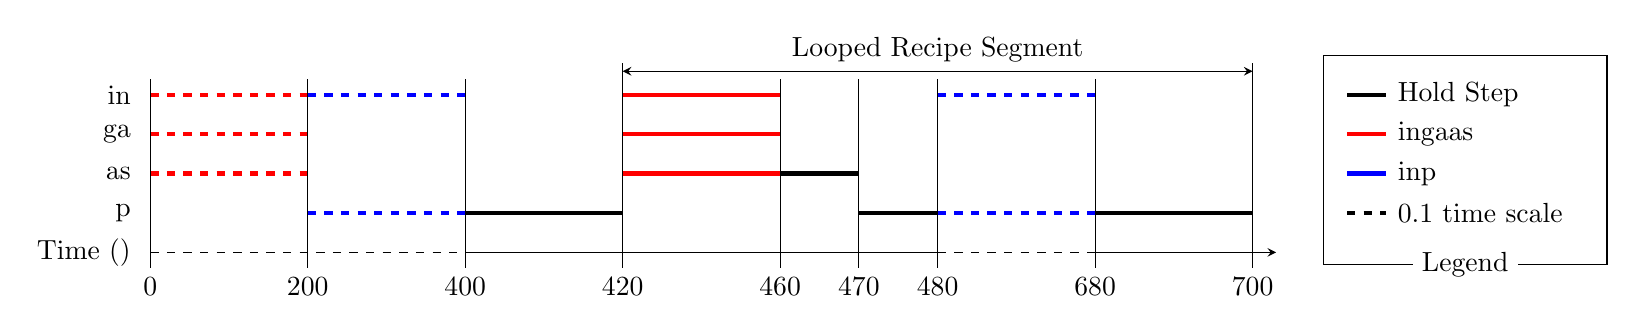
\begin{tikzpicture}
    \begin{scope}
    % lines
        \node [label={[label distance=0]180:\acs{in}}] at (0, 0) {};
        \draw [red, ultra thick, dashed] (0, 0) -- (2, 0); %/10
        \draw [blue, ultra thick, dashed] (2, 0) -- (4, 0); %10
        \draw [red, ultra thick] (6, 0) -- (8, 0);
        \draw [blue, ultra thick, dashed] (10, 0) -- (12, 0); %10
        %\draw [red, ultra thick] (7.35, 0) -- (8.1, 0);
        
        \node [label={[label distance=0]180:\acs{ga}}] at (0, -0.5) {};
        \draw [red, ultra thick, dashed] (0, -0.5) -- (2, -0.5cm); %/10
        \draw [red, ultra thick] (6, -0.5) -- (8, -0.5);
        
        \node [label={[label distance=0]180:\acs{as}}] at (0, -1) {};
        \draw [red, ultra thick, dashed] (0, -1) -- (2, -1); %/10
        \draw [red, ultra thick] (6, -1) -- (8, -1);
        \draw [ultra thick] (8, -1) -- (9, -1);
        
        \node [label={[label distance=0]180:\acs{p}}] at (0, -1.5) {};
        \draw [blue, ultra thick, dashed] (2, -1.5) -- (4, -1.5); %/10
        \draw [ultra thick] (4, -1.5) -- (6, -1.5);
        \draw [ultra thick] (9, -1.5) -- (10, -1.5);
        \draw [blue, ultra thick, dashed] (10, -1.5) -- (12, -1.5); %/10
        \draw [ultra thick] (12, -1.5) -- (14, -1.5);
        
    % labels and markers for the timescale
        \node [label={[label distance=0]180:Time (\second)}] at (0, -2) {};
        \draw [dashed] (0, -2) -- (4, -2);
        \draw [] (4, -2) -- (10, -2);
        \draw [dashed] (10, -2) -- (12, -2);
        \draw [-stealth] (12, -2) -- (14.3, -2); % +0.3
        \draw [] (0, 0.2) -- (0, -2.2) node[anchor = north] {\num{0}};
        \draw [] (2, 0.2) -- (2, -2.2) node[anchor = north] {\num{200}};
        \draw [] (4, 0.2) -- (4, -2.2) node[anchor = north] {\num{400}};
        \draw [] (6, 0.4) -- (6, -2.2) node[anchor = north] {\num{420}};
        \draw [] (8, 0.2) -- (8, -2.2) node[anchor = north] {\num{460}};
        \draw [] (9, 0.2) -- (9, -2.2) node[anchor = north] {\num{470}};
        \draw [] (10, 0.2) -- (10, -2.2) node[anchor = north] {\num{480}};
        \draw [] (12, 0.2) -- (12, -2.2) node[anchor = north] {\num{680}};
        \draw [] (14, 0.4) -- (14, -2.2) node[anchor = north] {\num{700}};
        \draw [stealth - stealth] (6, 0.3) -- (14, 0.3) node[midway, anchor=south] {Looped Recipe Segment};
    \end{scope}
    \begin{scope} [shift={(15.2cm, -0.5)}] % +0.9
        \draw [ultra thick] (0, 0.5) -- (0.5, 0.5) node[anchor = west, text=black] {Hold Step};
        \draw [red, ultra thick] (0, 0) -- (0.5, 0) node[anchor = west, text=black] {\acs{ingaas}};
        \draw [blue, ultra thick] (0, -0.5) -- (0.5, -0.5) node[anchor = west, text = black] {\acs{inp}};
        \draw [dashed, ultra thick] (0, -1) -- (0.5, -1) node[anchor = west, text = black] {\num{0.1} time scale};
        \draw (-0.3, 1) -- (3.3, 1) -- (3.3, -1.65) -- node[midway, fill = white] {Legend} (-0.3, -1.65) -- cycle;
    \end{scope}
    \end{tikzpicture}
    }
    \subcaptionbox{
    \acs{bf}-\acs{stem_m} overview images of two nanowires from sample 4. The wire on the left was cut with a regular cross-section, while the wire on the right was cut with a \qty{30}{\degree} cross-section.
    \label{subfig:s4_OV}
    }{
    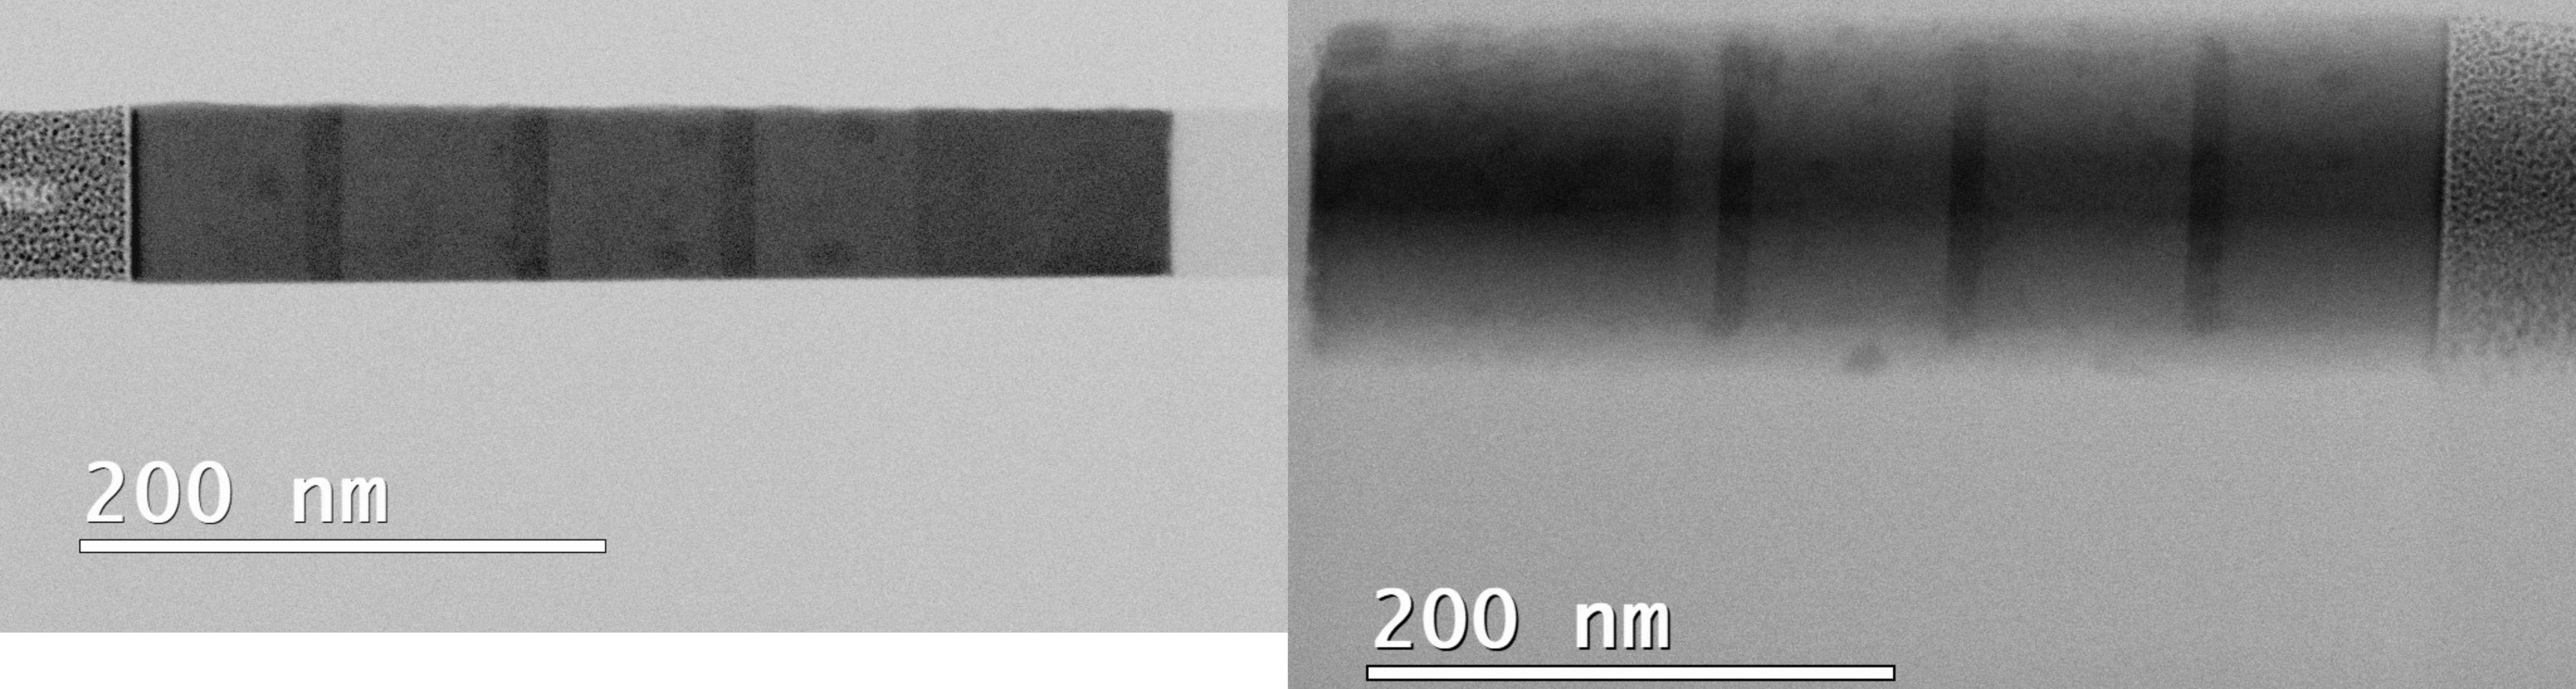
\includegraphics[width = 0.48\textwidth]{4_Crystalline_properties/Fig/s4_OV.pdf}
    }
    \subcaptionbox{
    High-resolution \acs{bf}-\acs{stem_m} images of the first \acl{qw} for both wires in \subref{subfig:s4_OV} with \acs{fft} inserts.
    \label{subfig:s4_HR}
    }{
    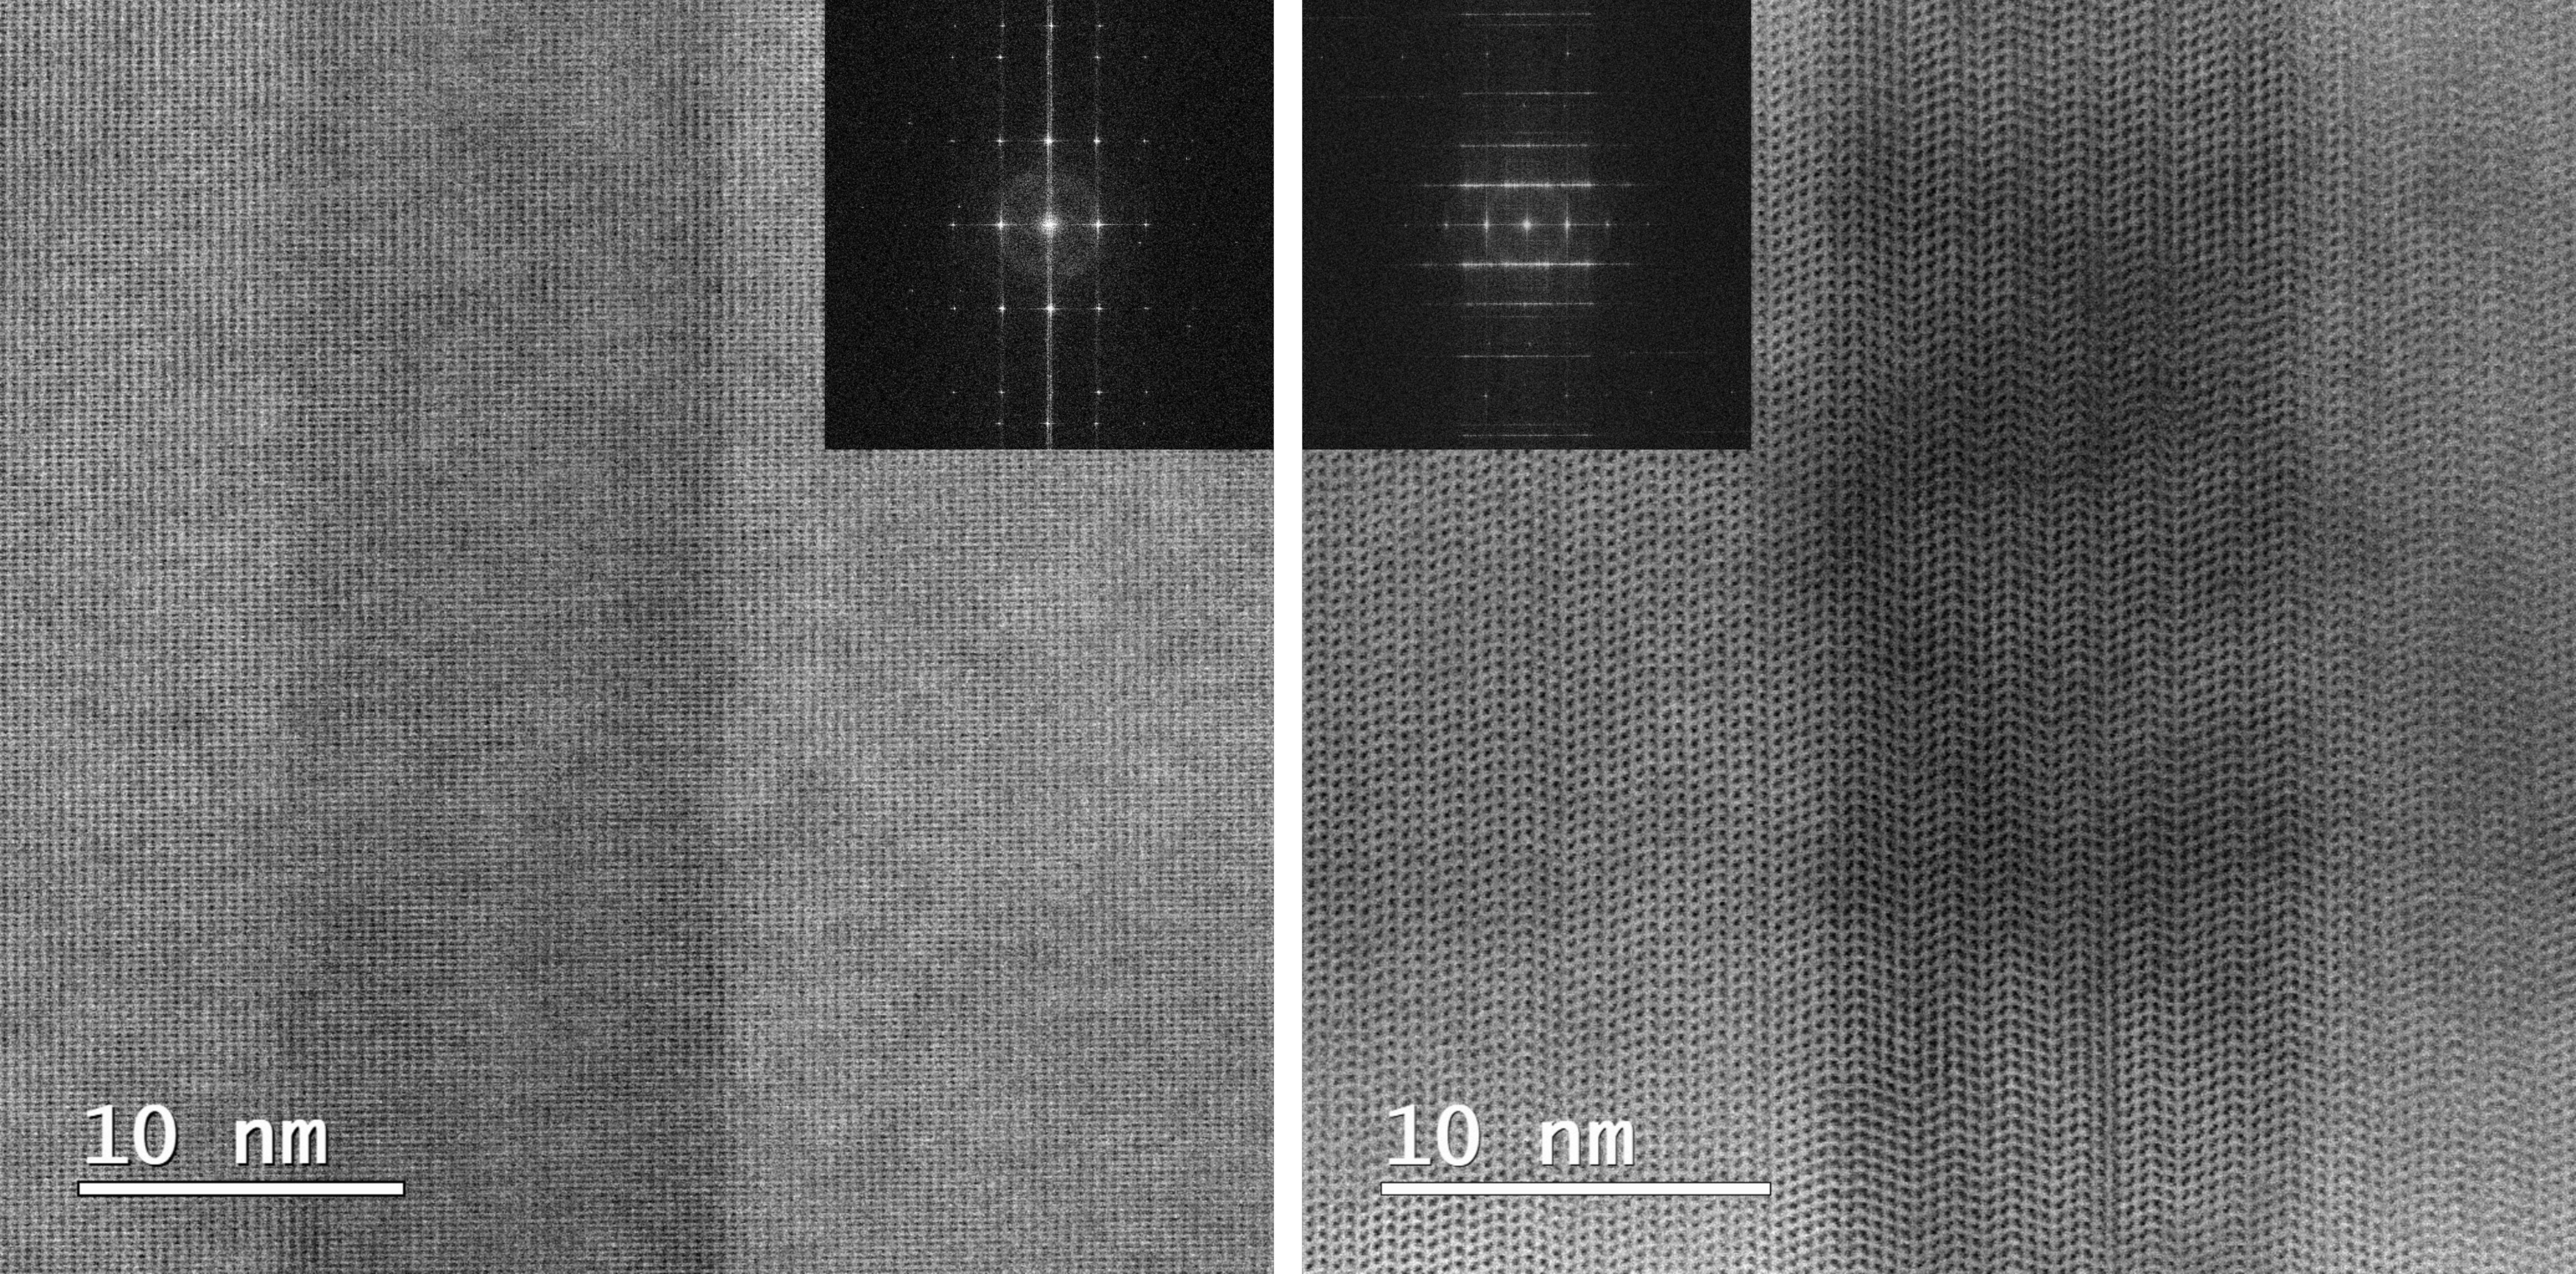
\includegraphics[width = 0.48\textwidth]{4_Crystalline_properties/Fig/s4_HR.pdf}
    }
    \caption{Growth recipe and \acs{bf}-\acs{stem_m} images of sample 4. The III-V material appears dark due to channelling contrast, with \acs{ingaas} being the darkest of the two III-V materials. \subref{subfig:recipe4} shows the growth recipe. \subref{subfig:s4_OV} shows overview images of the normal cross-section and \qty{30}{\degree} cross-section. \subref{subfig:s4_HR} shows high-resolution images of the first \acl{qw} for both wires in \subref{subfig:s4_OV} with inserts showing the calculated \acs{fft}s}
    \label{fig:s4_recipe_STEM}
\end{sidewaysfigure}

The recipe in Figure~\ref{subfig:recipe4} was kept similar to that used in sample 3 (Figure~\ref{subfig:recipe3}) for the initial experiment on the new \hkl<1 1 0> substrate. It contains a looped segment for creating \acs{ingaas} \acl{qw}s between \acs{inp} barrier layers. The main adjustments concern the deposition times. The initial growth steps, were changed from \qty{480}{\second} and \qty{180}{\second} to \qty{200}{\second} for both \acs{ingaas} and \acs{inp}, respectively. The deposition times for \acs{ingaas} \acl{qw}s were lowered from \qty{30}{\second} to \qty{20}{\second} in anticipation of the smaller area of the growth front. Simultaneously, the duration of \acs{inp} barrier steps was increased from \qty{180}{\second} to \qty{200}{\second}.

The most significant change concerned the post-\acs{ingaas} hold step. Here, \acs{as} precursor flow step time was reduced from \qty{15}{s} to \qty{10}{s} and the following \acs{p} precursor flow step time increased from \qty{5}{s} to \qty{10}{s}. This change was made to address the \acs{as} profile seen in the \acs{inp} layer of the sample 3 (Figure~\ref{subfig:s3_V_linesc}). By reducing the \acs{as} precursor flow time in the hold step it was hoped that the \acs{as} contamination in the first nanometres of the \acs{inp} layer would be reduced or, in the best case, eliminated in sample 4.

\subsection{Structural Analysis}

Figure~\ref{fig:s4_recipe_STEM} shows \acs{bf}-\acs{stem_m} images of two different wires from sample 4. The images on the left side of both Figure~\ref{subfig:s4_OV} and \ref{subfig:s4_HR} show the wire cut with a standard cross-section used in the previous chapter and schematised in Figure~\ref{subfig:FIB_cut_strategy}. In comparison, on the right side of the same figures, the images of a lamella cut with the \qty{30}{\degree} cross-section illustrated on the right of Figure~\ref{fig:110_FIB} are shown. 

Both lamellae come from the same sample, with identical device layer thickness. 
However, Figure~\ref{subfig:s4_OV} highlights how the \qty{30}{\degree} cross-section appears larger because the viewing angle is not perpendicular to the heterointerfaces that lay in the wafer plane. This distortion becomes clear when one looks at the III-V-\acs{si} interfaces at the top and bottom of the nanowires. The well-defined lines in the standard cross-section become large regions in the \qty{30}{\degree} cross-section. In these regions, the III-V nanowire and the \acs{sio2} template appear superimposed, as they are one on top of the other in the path the electron beam takes through the lamella.

An evident advantage of the \qty{30}{\degree} cut in combination with the \hkl<1 1 0> wafer is that vertical \hkl{1 1 1} heterointerfaces remain perpendicular to the viewing direction. As the recipe optimised in Chapter~\ref{chap:growth} stabilises this facet family, this new viewing angle does not affect the observer's ability to evaluate the sharpness of this type of interface from \acs{stem_m} measurements.

The comparison between the two wires at high resolution in Figure~\ref{subfig:s4_HR} also highlights the amount of structural information available when viewing a \hkl{1 1 0} plane (on the right) compared to a \hkl{1 1 2} plane (on the left). The presence of \acs{rtp}s is evident in the \qty{30}{\degree} cross-section both in the \acs{bf}-\acs{stem_m} image and in its \acf{fft} in the insert. The \acs{rtp}s have manifested as horizontal lines in the frequency domain. In contrast, both the \hkl{1 1 2} \acs{bf}-\acs{stem_m} image and its \acf{fft} do not contain any trace of this type of defect.

Both samples grew from silicon seeds that appear (in print) towards the centre of the image and grew out toward the margins. The initial \acs{ingaas} nucleation layer gives way to a lighter \acs{inp} layer in both lamellae, however, the length of this layer appears different. This could be due to a different shape of the nucleation \acs{ingaas}'s growth front. A trace of the complexity of this interface is seen at the bottom of the first well of the \qty{30}{\degree} cross-section. The bottom of this heterostructure appears bent towards the seed, suggesting that the \acs{inp} layer did not have enough time to grow to annihilate all the non-\hkl{1 1 1} facets.

\begin{table}[]
    \centering
    \caption{Growth rates for each heterolayer in the two nanowires in Figure~\ref{fig:s4_recipe_STEM}}
    \begin{tabular}{l|c c}
         & \multicolumn{2}{c}{growth rates (\nmmin)} \\
        heterolayer & \qty{0}{\degree} cross-section & \qty{30}{\degree} cross-section \\ \hline
        \acs{ingaas} nucleation & \num[separate-uncertainty=true]{29.0 (0.2)} & \num[separate-uncertainty=true]{42.4 (0.3)} \\
        \acs{inp} stabilisation & \num[separate-uncertainty=true]{18.3 (0.1)} & \num[separate-uncertainty=true]{4.7 (0.2)} \\ \hline
        \textbf{pre-wells layers} & \textbf{\num[separate-uncertainty=true]{23.7 (0.1)}} & \textbf{\num[separate-uncertainty=true]{23.6 (0.3)}} \\ \hline
        \acs{ingaas} well 1 & \num[separate-uncertainty=true]{39 (1)} & \num[separate-uncertainty=true]{35 (2)} \\
        \acs{inp} barrier 1 & \num[separate-uncertainty=true]{19.7 (0.2)} & \num[separate-uncertainty=true]{22.4 (0.1)} \\
        \acs{ingaas} well 2 & \num[separate-uncertainty=true]{41 (1)} & \num[separate-uncertainty=true]{38 (1)} \\
        \acs{inp} barrier 2 & \num[separate-uncertainty=true]{19.7 (0.2)} & \num[separate-uncertainty=true]{23.6 (0.1)} \\
        \acs{ingaas} well 3 & \num[separate-uncertainty=true]{43 (1)} & \num[separate-uncertainty=true]{39.1 (0.9)} \\
        \acs{inp} barrier 3 & \num[separate-uncertainty=true]{20.0 (0.2)} & \num[separate-uncertainty=true]{25.0 (0.1)} \\ \hline
        \textbf{wire total} & \num[separate-uncertainty=true]{22.5 (0.2)} & \num[separate-uncertainty=true]{24.4 (0.2)} \\ \hline \hline
    \end{tabular}
    \label{tab:s4_growth_rates}
\end{table}

\paragraph{Growth rates} The growth rates for each material layer in the wires of Figure~\ref{fig:s4_recipe_STEM} are summarised in Table~\ref{tab:s4_growth_rates}. These values were calculated by taking seven repeated measurements of each layer thickness perpendicularly to each heterointerface and are therefore comparable to the \hkl{1 1 1} growth rates of sample 3 (Table~\ref{tab:sample3_growth_rates}).

The discrepancy between the size of the \acs{ingaas} and \acs{inp} pre-well layers noted in the \acs{bf}-\acs{stem_m} images of the two wires from sample 4 is also reflected in their growth rates. The \acs{ingaas} growth rate for the nanowire observed with a \qty{30}{\degree} cross-section is \qty[separate-uncertainty=true]{42.4 (0.3)}{\nano\metre\per\minute}: significantly higher than that of its counterpart in the nanowire observed under the standard cross-section which stands at \qty[separate-uncertainty=true]{29.0 (0.2)}{\nano\metre\per\minute}. The \acs{inp} growth rates, however, have an opposite trend, resulting at \qty[separate-uncertainty=true]{4.7 (0.2)}{\nano\metre\per\minute} and \qty[separate-uncertainty=true]{18.3 (0.1)}{\nano\metre\per\minute}, respectively. 

Consequently, when examining the total growth rate of the nanowires before the first \acl{qw} the two values are within each other's error at \qty[separate-uncertainty=true]{23.6 (0.3)}{\nano\metre\per\minute} and \qty[separate-uncertainty=true]{23.7 (0.1)}{\nano\metre\per\minute}, respectively. Since the amount of material introduced in the reactor was the same for both wires, this would support the theory that a complex growth front forms in one of the two wires and then is simplified to a single \hkl{1 1 1} facet by the \acs{inp} layer. In this scenario \acs{inp} and \acs{ingaas} layers could be one behind the other in the path of the electron beam. Another option is that the "missing" \acs{inp} could have been removed during the \acs{fib} thinning of the lamella. During this process, part of the nanowire's material is removed; therefore, the III-V semiconductor film seen in the \acs{stem_m} image is only a portion of the entire wire.

Both the \acs{ingaas} well and \acs{inp} growth rates increase as the growth front approaches the opening of the template. This trend is not very pronounced for the \acs{inp} layers of the nanowire cut with the standard cross-section procedure but is more pronounced in the \qty{30}{\degree} cross-section sample. This results in a higher total growth rate for the latter nanowire, with nearly \qty{2}{\nano\metre\per\minute} of difference. This difference, which develops in the latter precursor-switching-rich part of the recipe when the growth front is nearer to the template opening, could indicate a limited competition between neighbouring nanowires or a precursor concentration gradient in the reactor in the moments immediately following the precursor switches.
\par

\subsection{Compositional analysis}

\begin{figure}
    \centering
    \subcaptionbox{
        III-element \acs{eds} map. Red \acs{in}, blue \acs{ga}
        \label{subfig:s4_0deg_IIImap_wells}
        }{
        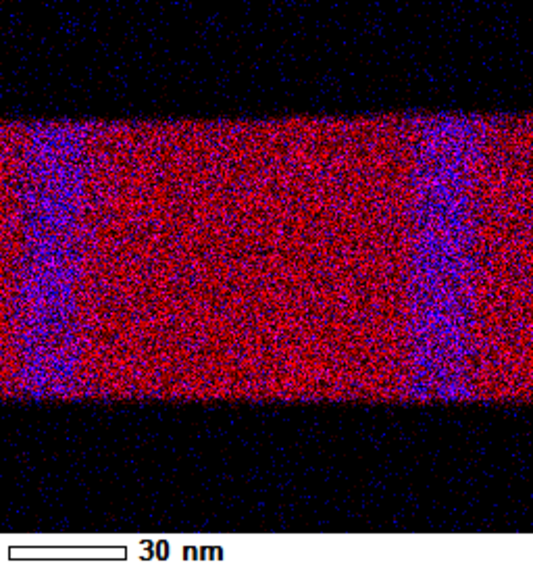
\includegraphics[width=0.48\textwidth]{4_Crystalline_properties/Fig/s4_0deg_IIImap_wells.pdf}
    }
    \subcaptionbox{
        V-element \acs{eds} map. Red \acs{as}, blue \acs{p}
        \label{subfig:s4_0deg_Vmap_wells}
        }{
        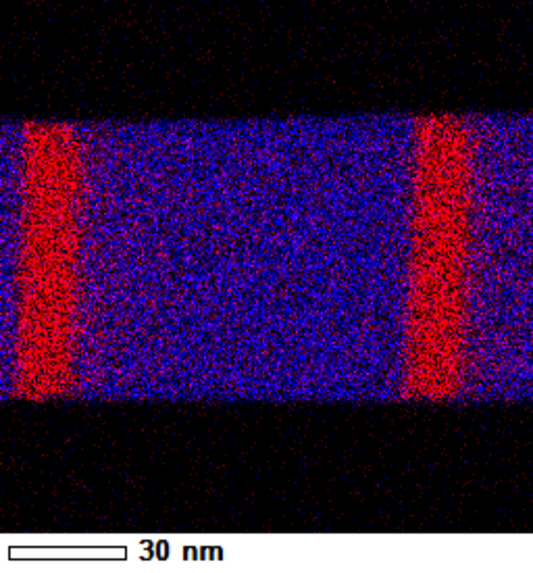
\includegraphics[width=0.48\textwidth]{4_Crystalline_properties/Fig/s4_0deg_Vmap_wells.pdf}
    }
    \caption{\acs{eds} maps of the \acl{qw} region of the \qty{0}{\degree} sample in Figure~\ref{subfig:s4_OV}. The seed is out of frame on the left of the images.}
    \label{fig:s4_0deg_EDS_maps_wells}
\end{figure}

Figure~\ref{fig:s4_0deg_EDS_maps_wells} shows the \acs{eds} maps. The elements \acl{ga} and \acl{p} are colour-coded in blue while \acl{in} and \acl{as} are colour-coded in red. Two \acs{ingaas} \acl{qw}s are visible on both maps, showing the same nanowire area. 

The III-element map shows how \acl{ga} is well-segregated into the \acs{ingaas} layers. However, a difference between the leading and trailing edges of the \acl{qw}s is visible once more when examining the V-element map. Indeed, while the leading edge is sharp, a light red shading is present in the \acl{p} region after the trailing edge. This indicates an \acl{as} contamination in the \acs{inp} barrier layer. As the image is comparable to the one in Figure~\ref{subfig:s3_V_map_wells}, the lengthening of the \acs{p} flow step during the post \acs{ingaas} hold step had a small impact on the resulting post-well composition profile.

\begin{figure}
    \centering
    \subcaptionbox{
    \acs{eds} linescan: III atomic percentage vs position.
    \label{subfig:s4_III_0deg_linesc}
    }{\begin{tikzpicture}
        \begin{axis}[
            width = 0.8\textwidth,
            height = 5cm,
            xlabel = Position (nm),
            ylabel = Composition (atomic \%),
            table/col sep=comma,
            %title = III element composition,
            legend pos=outer north east,
            ymin=0, ymax=100,
            xmin = 0, xmax=230
        ]
    \addplot [cb1_orange,] table[x=nm,y=Ga] {4_Crystalline_properties/csv/s4_III_0deg_linesc.csv};
    \addplot [cb1_dark_blue,] table[x=nm,y=In] {4_Crystalline_properties/csv/s4_III_0deg_linesc.csv};
    \addlegendentry{Ga}
    \addlegendentry{In}
    \end{axis}

    \end{tikzpicture}
    }
    \subcaptionbox{
    \acs{eds} linescan: V atomic percentage vs position.
    \label{subfig:s4_V_0deg_linesc}
    }{\begin{tikzpicture}
        \begin{axis}[
            width = 0.8\textwidth,
            height = 5cm,
            xlabel = Position (nm),
            ylabel = Composition (atomic \%),
            table/col sep=comma,
            %title = V element composition,
            legend pos=outer north east,
            ymin=0, ymax=100,
            xmin = 0, xmax=230
        ]
    \addplot [cb1_orange,] table[x=nm,y=As] {4_Crystalline_properties/csv/s4_V_0deg_linesc.csv};
    \addplot [cb1_dark_blue,] table[x=nm,y=P] {4_Crystalline_properties/csv/s4_V_0deg_linesc.csv};
    \addlegendentry{As}
    \addlegendentry{P}
    \end{axis}

    \end{tikzpicture}
    }
    \caption{\acs{eds} linescan compositional data (in percentage) for the \subref{subfig:s4_III_0deg_linesc} III elements and \subref{subfig:s4_V_0deg_linesc} V elements across all three \acl{qw} of the \qty{0}{\degree} sample seen in Figure~\ref{subfig:s4_OV}. The origin of the x-axis is situated before the first well and is the closest point to the \acs{si} seed. Higher position numbers (in nm) represent the scan moving along the \hkl{1 1 1} vector perpendicular to the growth front away from the seed.}
    \label{fig:s4_0deg_linescans}
\end{figure}

Figure~\ref{fig:s4_0deg_linescans} shows the composition data calculated from the \acs{eds} linescan taken on the \acl{qw} region of the \qty{0}{\degree} sample in Figure~\ref{subfig:s4_OV}. The scan was taken from before the first \acl{qw}, closest to the \acs{si} seed.

The III-element composition profile of Figure~\ref{subfig:s4_III_0deg_linesc} was calculated using the L\(_\alpha\) lines of \acl{in} and \acl{ga}. The graph is very noisy, with noise fluctuations reaching \qty{20}{\%}, but shows a composition close to \ce{In0_.4Ga0_.6As} in all three \acl{qw}s. Similarly to the profile in Figure~\ref{subfig:s3_III_linesc}, suggests the presence of a \acl{ga} composition gradient after the well itself. 

The V-element composition profile of Figure~\ref{subfig:s4_V_0deg_linesc} was calculated using the K\(_\alpha\) lines of \acl{as} and \acl{p}. This graph has noise fluctuations of about \num{10}-\qty{15}{\%}. A \acl{as} percentage composition close to \qty{100}{\%} is present in the \acs{ingaas} \acl{qw} similarly to what was observed for sample 3 (Figure~\ref{subfig:s3_V_linesc}). The \acs{as}-rich region extends for \num{10}-\qty{15}{\nano\metre} after the end of the \acs{ingaas} \acl{qw}.

As the precursor flows were not altered from those of previous samples, the V / III ratios remain as in Table~\ref{tab:sample1_ratios}. The higher concentration of \acl{ga} in the \acl{qw}s could therefore be caused by the change in the geometry of the template given by the difference in device layer thickness of the \hkl<1 1 0> \acs{soi} wafer.

\subsection{Photoluminescence data}

\begin{figure}
    \centering
    \begin{tikzpicture}
        \begin{axis}[
            width = 0.8\textwidth,
            height = 5cm,
            xlabel = Wavelegth (nm),
            ylabel = Intensity (A.U.),
            table/col sep=comma,
            %title = Photoluminescence Spectrum,
            legend pos=outer north east,
            ymin=0, ymax=100,
            xmin = 1268.8, xmax=1600.3
        ]
    \addplot [cb1_dark_blue,] table[x=Wavelength,y=Intensity] {4_Crystalline_properties/csv/s4_pl.csv};
    \addlegendentry{In}
    \end{axis}
    \end{tikzpicture}
    \caption{Caption}
    \label{fig:s4_pl}
\end{figure}




\section{Minimization of Nucleation Layer Thickness}




\section{Merge Structures}





\section{Growth of Strained Heterolayers}







%\section{article1}
%\begin{figure}
%    \centering
%    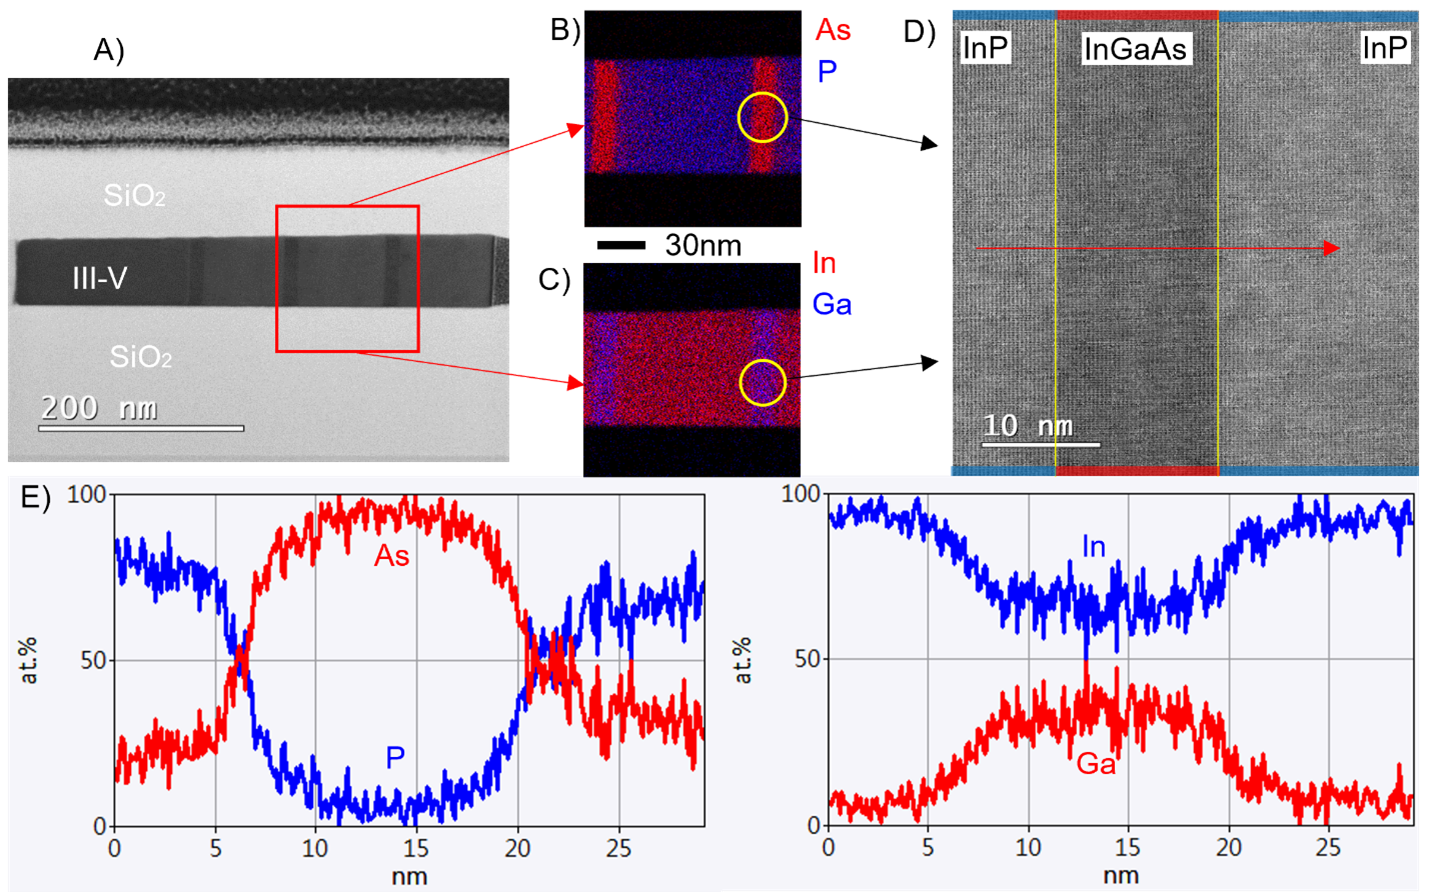
\includegraphics[width=\textwidth]{3_Growth/ICMOVPEXXFig5.png}
%    \caption{STEM image and EDS maps of a lamella cut from one of the nanowires grown on a <110> SOI. A) Overview of the BF-STEM image of the nanowire. The silicon seed is on the left, and silicon oxide is on the top and bottom. The entire heterostructure stack is visible due to channelling contrast: InGaAs appear darker than InP. B) Color-coded EDS map of the region highlighted by the red square in (A): in red In concentration and blue Ga concentration. C) Color-coded EDS map of the region highlighted by the red square in (A): red As concentration and blue P concentration. D) High-resolution BF-STEM detail of the 10-nm-thick InGaAs well. E) EDS line-scan spectra recorded across the InGaAs and highlighted in (D) by the red arrow showing scan direction.}
%    \label{fig:ICMOVPEXXFig5}
%\end{figure}

%In the previous examples, a <001> device layer SOI was used as a growth substrate, where a multi-faceted growth front can develop, leading to poor geometric control, composition variations for ternaries, and in any case, a heterointerface which is not perpendicular to the growth direction, which is an undesirable situation for device fabrication. This can be circumvented using a Si wafer orientation with vertical {111} crystal planes as available on an <110> SOI wafer—

%hfigure 5. A shows a BF-STEM image of a nanowire with vertical and well-defined hetero-interfaces. 

%A similar level of As background impurities is present after each InGaAs segment, as shown in Figure 5. B, while Figure 5. C shows how Ga is well confined to the respective layer. 

%The high-resolution BF-STEM image in Figure 5.D shows the heterointerface between the 85-nm-thick InP on the image's left- and right-hand side and the 14-nm-thick InGaAs quantum well structure that appears as a dark layer in the middle of the image. The extracted <111>B growth rates are 25.5 nm/min for InP and 42.9 nm/min for InGaAs, respectively. This marks an increase in growth rate attributed to the different template shapes, as template height was reduced from 220 nm to 70 nm—

%figure 5. E shows the composition profiles for the III- and group elements across the quantum well region. The presence of As impurities immediately after the quantum well layer is again noticeable on the right side of the V element map, as the As and P concentration profiles are asymmetric. This asymmetry is evident when compared with the symmetric composition profiles for the III-group elements, which maintain the interface quality observed in the sample shown in Figure 4. The III composition profile Figure 5. E highlights how the InxGa1-xAs composition is more prosperous in Indium, having an x = 0.60. As the flows into the reactor were not altered from the sample shown in Figure 4, this composition change can also be attributed to the different template geometry.

\section{article 2}
\begin{figure}
    \centering
    \includegraphics[width=\textwidth]{4_Crystalline_properties/From_Article2/Figure2.png}
    \caption{Top-view SEM images of arrays with grown III-V nanowires. The \qty{70}{\nm}, \qty{140}{\nm}, \qty{210}{\nm}, and \qty{280}{\nm} wide wires are shown from top to bottom. The arrays on the left contain structures grown from a seed surface parallel to the template direction, while those on the right are grown from seed surfaces that are tilted concerning the template. On the bottom left of the images, the three main elements of the arrays are highlighted in green (silicon seed), red (III-V nanowires), and blue (template opening).}
    \label{fig:arrays}
\end{figure}

Figure~\ref{fig:arrays} shows growth results from sample 1 of arrays containing template nanotubes of four different widths (\qty{70}{nm}, \qty{140}{nm}, \qty{210}{nm}, and \qty{280}{nm}). Each array contains 66 nanowires (in red) grown from silicon (in green) and arranged in 33 pairs. Each pair of wires shares the same template opening (in blue). 
\par
Each wire in the array can be identified by its row, opening, and position relative to the latter. Each row is numbered from 1 to 11, starting at the bottom of the array. The template openings are marked by letters A, B, or C; the wires connected to the opening to the left (l) or right (r) can be easily distinguished. Therefore, a string such as 9Br identifies a single wire in the array. 
\par
Our growth methodology aims to select and maintain a single \hkl{111}\(_B\) facet as the nanowire's growth front. If a III-V wire end-surface is multi-faceted or not parallel to the \acs{si} seed facet, the wire is classified as defective in this study without requiring a further in-depth STEM analysis. This first distinction allows the evaluation of the fraction of "perfect" wires, defining a growth yield. 
\par
In Figure~\ref{fig:arrays}, the \qty{280}{nm} tilted arrays present some defective wires in 11Al, 6Cr, and 7Cr; however, the other wires in each pair (11Ar, 6Cl, and 7Cl) appear “perfect”. As is evident in the case of wire 6Cr, the wire grew into an unpredictable shape after nucleation. It is unclear if the source of defective wires can be attributed solely to the nucleation step, as there are other sites (\qty{70}{nm} tilted 6Cl, \qty{140}{nm} perpendicular 2Br, 11Br, and \qty{280}{nm} perpendicular 7Br) that present a defective wire and fully covered seed. However, this finding suggests that nucleation does play an important role in the following growth facet selection.


\begin{figure}
    \centering
    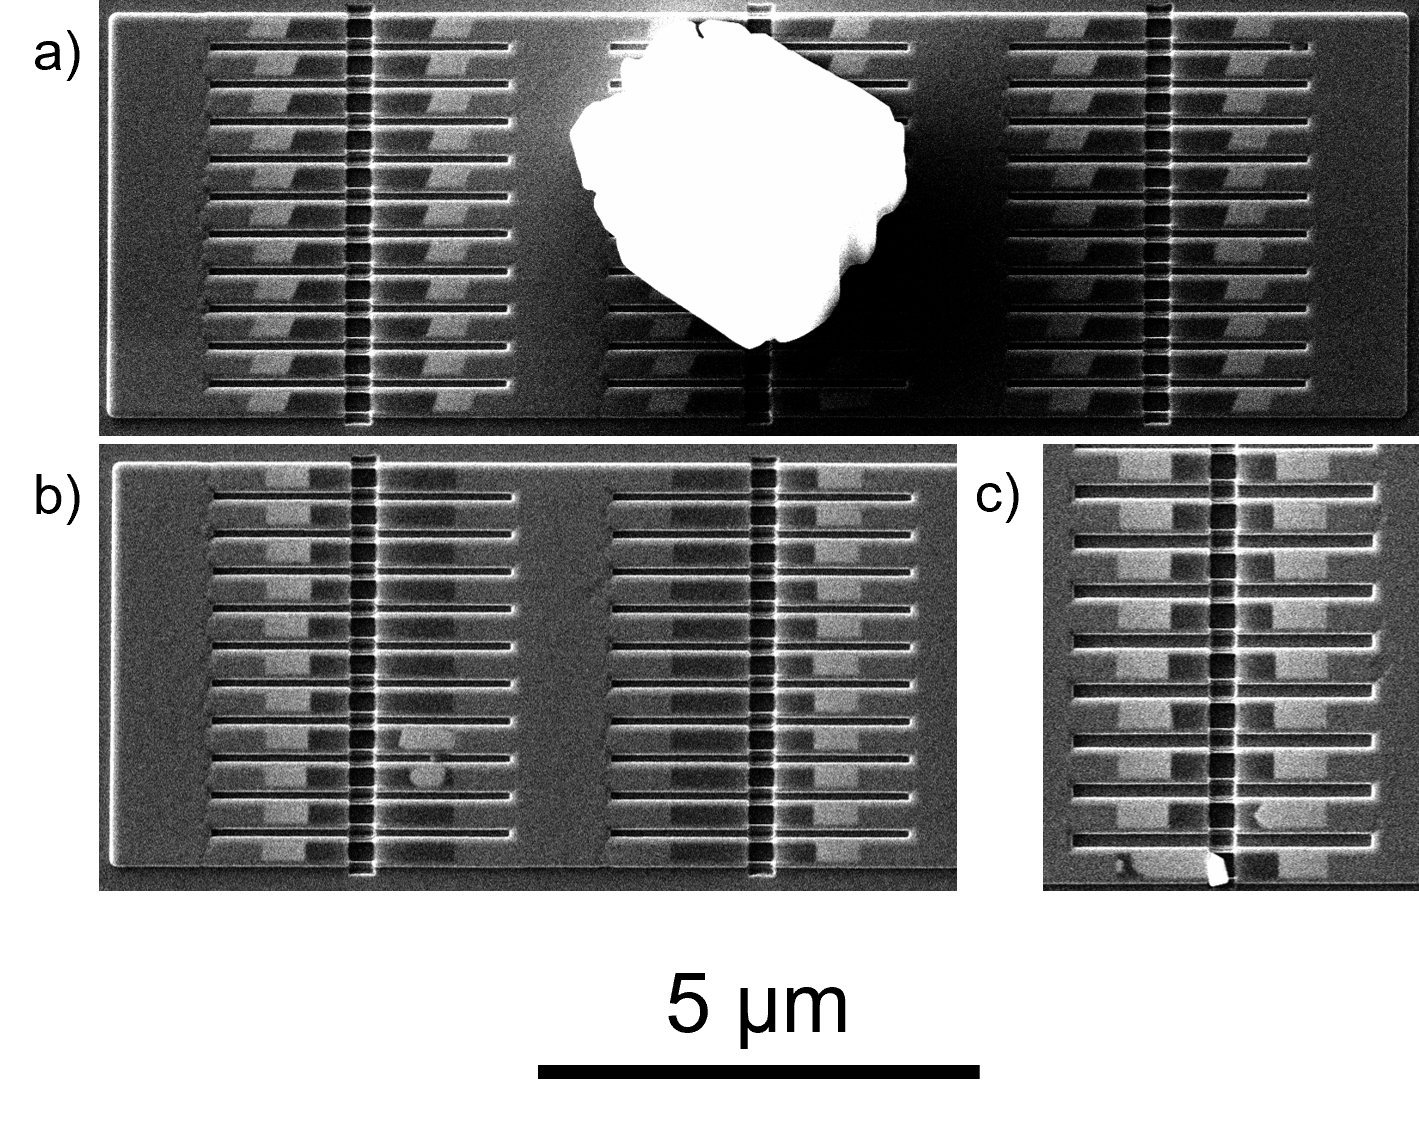
\includegraphics[width=\columnwidth]{4_Crystalline_properties/From_Article2/Figure3.png}
    \caption{Examples of failure situations for TASE grown wires. (a) large parasitic crystal obstructing many growth sites. (b) multiple seeds do not show nucleation of III-V material at all, while one site shows parasitic nucleation inside the template. (c) in the bottom row, after initial nucleation on the \acs{si}, a parasitic crystal developed inside the template and grew out of it.}
    \label{fig:failures}
\end{figure}

Another parameter that negatively affects the growth yield is the loss of growth selectivity and the resulting parasitic growth. This is ascribed to impurities or surface features promoting nucleation. An example of this is shown in Figure~\ref{fig:failures}.a, where a single defect of this kind affects many wires. Figure~\ref{fig:failures}.b also shows sites where parasitic nucleation occurred within templates and, seed-sites that did not undergo III-V on \acs{si} nucleation, likely because of the lingering of a passivating \acs{sio2} layer on the \acs{si} seed surface. This happened despite the proximity to other correctly-grown wires. Finally, 
Figure~\ref{fig:failures}.c bottom row illustrates an example where, after the initial nucleation event, the channel was obstructed by a parasitic nucleation growth within the channel, which extends outside the template. This type of growth configuration can potentially cause deposits similar to that in Figure~\ref{fig:failures}.a.

\subsection{Yield study}

\sisetup{detect-all = true}
\begin{table}
    \centering
    \begin{tabular}{l|ccccccc}
        \hline
         & \multicolumn{7}{c}{Defect categories and occurrence} \\ 
         & $\begin{matrix} \text{Wrong} \\ \text{Facet} \end{matrix}$ & $\begin{matrix} \text{Hidden by} \\ \text{Parasitic} \end{matrix}$ & $\begin{matrix} \text{Oxide} \\ \text{Nucleated} \end{matrix}$ & $\begin{matrix} \text{Seed} \\ \text{Exposed} \end{matrix}$ & Long & Short & Ungrown \\ 
        \hline \hline
         & & & & & & & \\
        Sample 1 & \num{164} & \num{230} & \num{2} & \num{0} & \num{5} & \num{204} & \num{61} \\ 
        \hline
        Parallel & \num{81} & \num{170} & \num{1} & \num{0} & \num{4} & \num{0} & \num{0} \\
        \textit{\% of category} & \textit{\qty{49.4}{\%}} & \textit{\qty{77.9}{\%}} & \textit{\qty{50}{\%}} & \textit{-} & \textit{\qty{80}{\%}} & \textit{\qty{0}{\%}} & \textit{\qty{0}{\%}} \\ 
        \hline
        Tilted & \num{83} & \num{51} & \num{1} & \num{0} & \num{1} & \num{204} & \num{61} \\
        \textit{\% of category} & \textit{\qty{50.6}{\%}} & \textit{\qty{22.1}{\%}} & \textit{\qty{50}{\%}} & \textit{-} & \textit{\qty{20}{\%}} & \textit{\qty{100}{\%}} & \textit{\qty{100}{\%}} \\ 
        \hline
         & & & & & & & \\
        Sample 2 & \num{204} & \num{257} & \num{15} & \num{8} & \num{3} & \num{7} & \num{20} \\ 
        \hline
        Parallel & \num{127} & \num{145} & \num{6} & \num{4} & \num{1} & \num{5} & \num{20} \\
        \textit{\% of category} & \textit{\qty{62.3}{\%}} & \textit{\qty{56.4}{\%}} & \textit{\qty{40}{\%}} & \textit{\qty{50}{\%}} & \textit{\qty{33.3}{\%}} & \textit{\qty{71.4}{\%}} & \textit{\qty{100}{\%}} \\ 
        \hline
        Tilted & \num{77} & \num{112} & \num{9} & \num{4} & \num{2} & \num{2} & \num{0} \\
        \textit{\% of category} & \textit{\qty{37.7}{\%}} & \textit{\qty{43.6}{\%}} & \textit{\qty{60}{\%}} & \textit{\qty{50}{\%}} & \textit{\qty{66.7}{\%}} & \textit{\qty{28.6}{\%}} & \textit{\qty{0}{\%}} \\ 
        \hline
        & & & & & & & \\
        \textbf{Total} & \textbf{\num{368}} & \textbf{\num{487}} & \textbf{\num{17}} & \textbf{\num{8}} & \textbf{\num{8}} & \textbf{\num{211}} & \textbf{\num{81}} \\
        \hline
    \end{tabular}
    \caption{Distribution of failure types for samples 1 and 2. Each sample's total is broken down between wires grown parallel to or tilted away from the \hkl<111> direction. Percentages for these two sub-categories and an overall total are given.}
    \label{tab:failures}
\end{table}
\sisetup{detect-none = true}

A survey of the arrays was carried out using samples 1 and 2, and involved \num{15840} individual nanowires grown in \num{240} arrays grouped in \num{5} locations per sample. The areas investigated were the top left of the chips as well as randomly selected locations throughout it. Wires need to have two parallel visible \hkl{111} seed and end facets of equal length, and they need to have nucleated directly on the \acs{si} seed covering it in its entirety for them to be considered "perfect". Of the \num{15840} total wires \num{14660} match these criteria, totalling a global yield of \qty{92.55}{\%}.
\par
Of the \num{7920} wires imaged for each sample, \num{7254} grew successfully in sample 1, and \num{7406} grew successfully in sample 2, resulting in a corresponding growth yield of \qty{91.59}{\%} and \qty{93.51}{\%}. This result indicates that the different heterointerfaces of samples 1 and 2 do not significantly impact the growth yield. 
\par
Further analysis was carried out within each sample by comparing the template growth yield parallel to the \hkl<111> direction, and those tilted away from it. A larger number (\num{9504} out of \num{15840}) of wires of the first configuration were measured. For sample 2, the parallel and tilted configurations resulted in comparable growth yields of \qty{93.73}{\%} and \qty{93.75}{\%}, while sample 1 showed \qty{94.84}{\%} and \qty{86.71}{\%} growth yields for the same configurations. The larger difference in growth yields for parallel and tilted templates in sample 1 can be explained by one of the fivcategorisedselected locations containing tilted arrays, falling in an area of the chip with many nucleation issues. This area is reflected in Table~\ref{tab:failures} where sample 1 has more short and ungrown wires.
\par
The total of \num{1180} nanowires that experienced growth failure are categorised based on the type of failure they experienced. Table~\ref{tab:failures} breaks down the number of defective wires for each sample between parallel and tilted templates, on a per-category basis. The first category, labelled "wrong facet", groups wires which terminate with either a multi-faceted surface or in a single facet that is not parallel to the seed surface, and accounts for \num{368} wires (\qty{31.2}{\%} of the total defective wires). The second and largest category comprises wire locations hidden by a parasitic crystal (\num{461} wires or \qty{39.0}{\%} of the total failures). From a total of \num{240} arrays, \num{32} are affected by one or more parasitic crystals. Still, the parasitic crystals hide close to \num{15} (\num{14.87} on average) locations for nanowire growth in each of these arrays. The "oxide nucleated" category contains all the cases where a III-V crystal nucleated randomly inside a template instead on the \acs{si} seed and counts \num{17} wires, \qty{1.4}{\%} of the total. The wires in the category "seed exposed" have the expected end facet, but did not fully cover the entire seed surface, leaving some of it exposed (\num{8} wires, \qty{0.7}{\%}). The category "long" comprises wires that were significantly longer than the others but did not have other defects, accounting for \qty{0.7}{\%} of the defective wires for a total of \num{8}. The last two categories are abnormally short wires and ungrown wires, with \num{211} (\qty{20.1}{\%}) and \num{81} (\qty{6.9}{\%}) counts each. These two categories of wires are more common in the area which presented nucleation iCharacterisation1.

\section{Growth rate stability and merging of nanostructures during growth}

\subsection{Heterointerfaces and growth rate in nanowires}

\begin{figure}
    \centering
    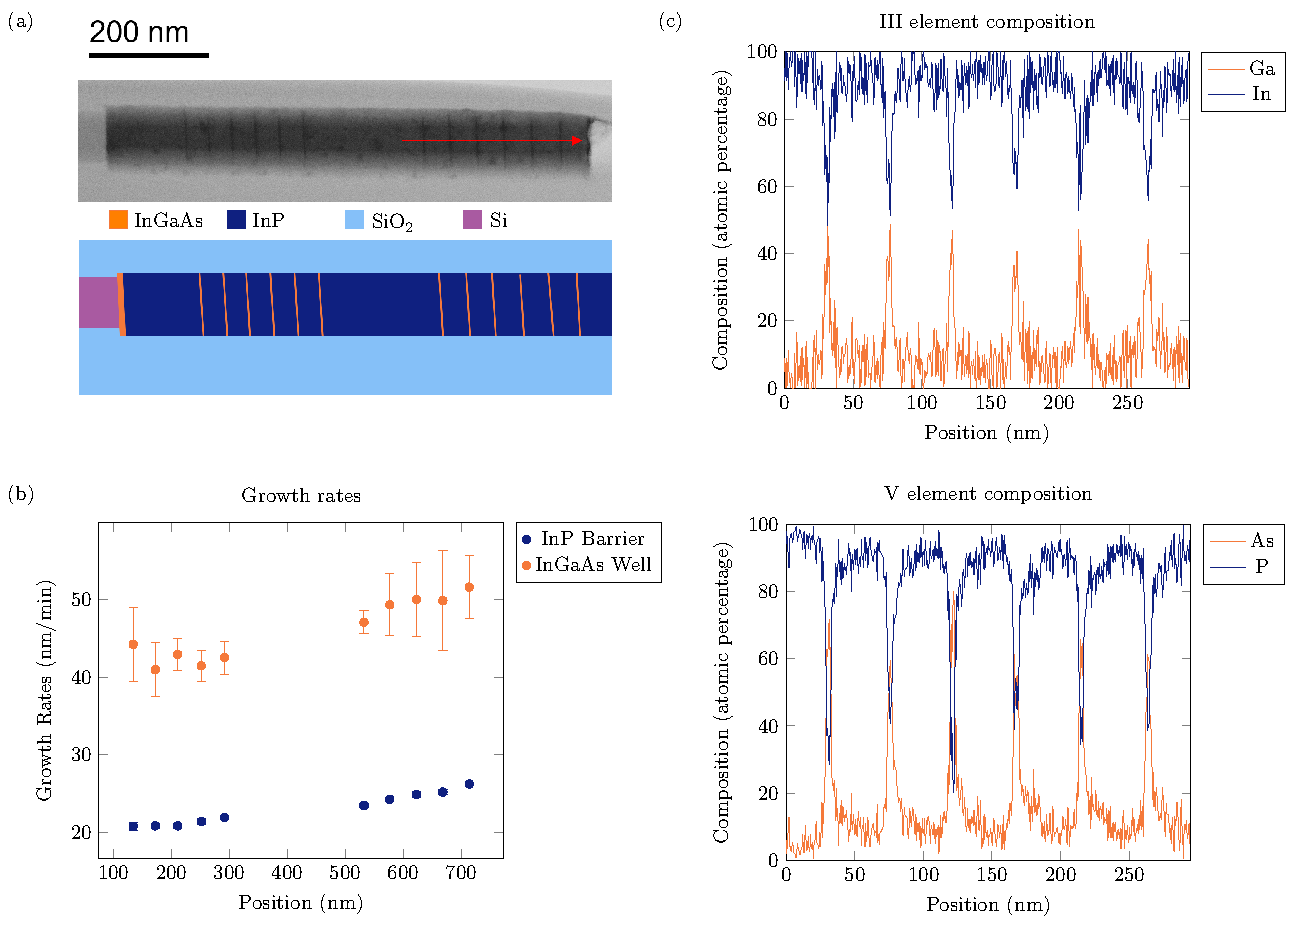
\includegraphics[width=\textwidth]{4_Crystalline_properties/From_Article2/Figure4.pdf}
    \caption{Characterisation results for sample 1. (a) BF-STEM image of the cross-section of one of the nanowires and corresponding schematic composition drawing. (b) growth rates of \acs{ingaas}, in orange, and \acs{inp}, in dark blue. Error bars on all x coordinates, and y coordinates of the \acs{inp} series, are smaller than the graphical markers. (c) composition profiles calculated from an EDS line scan recorded on the location and with the direction marked by the red arrow in (a).}
    \label{fig:growth_rates}
\end{figure}

An in-depth STEM and EDS analysis was carried out to assess the structure of the nanowires. Figure~\ref{fig:growth_rates}.a shows the STEM microscopy image of a FIB cross-section of a wire from sample 1. The blurred regions at the top and bottom are due to the \qty{30}{\degree} cut angle employed to access the \hkl<110> imaging direction. The \qty{4}{\nm} thin, on average, \acs{ingaas} segments are visible as twelve thin dark vertical lines in the dark grey body of the wire. The \acs{ingaas} layers cross-section also act as time markers, recording the morphology of the growth front, and revealing when a single facet is formed and maintained in the growth process. The slight tilt of the heterolayers, which do not appear to be perpendicular to the wafer surface, can partially be explained by a slight tilt of the device \acs{si} layer in this area of the wafer, as well as tilting due to a rotation of the crystalline growth axis during nucleation.
\par
Due to the presence of the \acs{sio2} template, the quantum wells only develop axially and not laterally. This translates into an enhanced composition control in ternary III-V compounds heterolayers incorporated in the nanowires \cite{Borg2019} and therefore is expected to allow for better control of the emission spectra. An EDS line scan of the last six \acs{ingaas} quantum wells was recorded along the direction indicated by the red arrow in Figure~\ref{fig:growth_rates}.a. The resulting composition profiles are shown in Figure~\ref{fig:growth_rates}.c, demonstrating consistent composition profiles across the wells, with the \acs{in} molar fraction being between \num{0.5} and \num{0.6}.
\par
A growth rate analysis is shown in Figure~\ref{fig:growth_rates}.b, revealing a variation in the \acs{inp} growth rate of around \qty{6}{\nm\per\minute} from \qty[separate-uncertainty=true]{20.7 (0.5)}{\nano\metre\per\minute} to \qty[separate-uncertainty=true]{26.2 (0.2)}{\nano\metre\per\minute} along \qty{600}{\nm} of wire. Similarly, a \qty{7}{\nano\metre\per\minute} growth rate increase was recorded for the \acs{ingaas} segments. The error bars represent the \qty{95}{\%} confidence interval on the measurement, calculated by averaging seven thickness measurements taken at various positions for each \acs{inp} and \acs{ingaas} segment. This growth rate increase shows a moderate influence of the diffusional process on the growth dynamics of the samples \cite{bjork2012}.

\begin{figure}
    \centering
    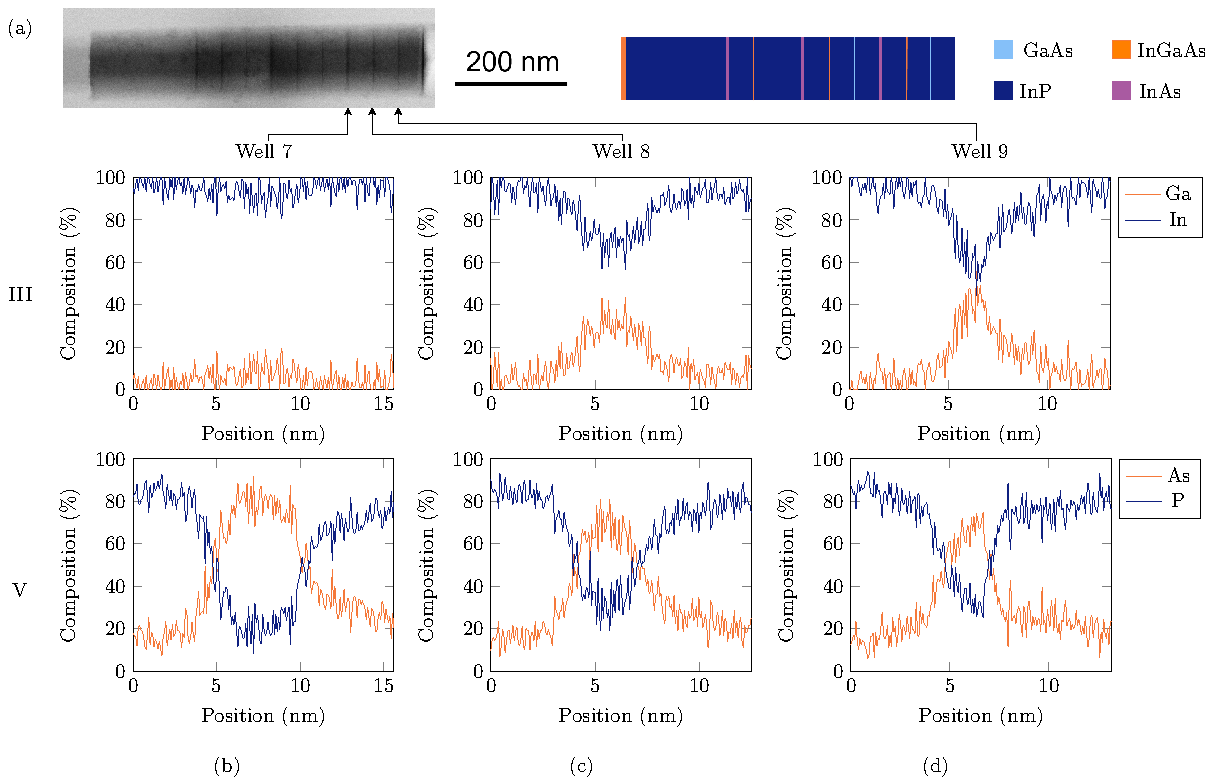
\includegraphics[width=\textwidth]{4_Crystalline_properties/From_Article2/Figure5.pdf}
    \caption{Analysis of sample 2. (a) BF-STEM image of the III-V nanowire, \num{9} lines corresponding to the arsenide layers and corresponding schematic drawing with coloured layers indicating the design composition. Composition profiles for the 7th (b), 8th (c), and 9th (d) wells are calculated from EDS line scans carried out across the respective quantum well from left to right, in the direction parallel to the growth axis.}
    \label{fig:composition}
\end{figure}

A STEM and EDS analysis of sample 2 was conducted to assess the structure and influence of strained heterointerfaces (Figure~\ref{fig:composition}.a) on the growth of nanowires containing three \acs{inp}-\acs{inas}-\acs{inp}-\acs{ingaas}-\acs{inp}-\acs{gaas} heterolayer sequences. Figure~\ref{fig:composition}.b shows the results of the \acs{inas} layer, where only the group V element precursor needs to be switched. The EDS profile indicates that this layer has formed as intended, with a phosphorus background level. 
\par
The \acs{ingaas} segment, with a target composition of \ce{In0_.53Ga0_.47As}, grew \acs{in}-rich, as seen from the EDS profiles in Figure~\ref{fig:composition}.c. A similar observation is made for the intended \acs{gaas} heterostructure: optimisation {fig:composition}.d shows this layer is heavily alloyed with a recorded \acs{in} molar fraction close to \num{0.5}. This indicates that the hold steps implemented in the growth recipe and designed to exhaust the group III element precursor (\acs{in}) were set too short. Further optimisation with prolongation of the purging step is thus suggested to improve composition control for these thin \qty{3}{nm}-wide heterostructures.
\par
The growth rates of the \acs{ingaas} and \acs{inp} layers were assessed with a process analogous to the one used for the growth rates of sample 1. The \acs{inp} growth rates is \qty[separate-uncertainty=true]{23.8 (0.3)}{\nano\metre\per\minute} between the first \acs{inas} and the first \acs{ingaas} wells and \qty[separate-uncertainty=true]{24.0 (0.4)}{\nano\metre\per\minute} between the third \acs{inas} and the third \acs{ingaas} wells. The \acs{ingaas} growth rates are \qty[separate-uncertainty=true]{39 (3)}{\nano\metre\per\minute} for the first \acs{ingaas} well and \qty[separate-uncertainty=true]{44 (2)}{\nano\metre\per\minute} for the third \acs{ingaas} well. All values are averaged from repeated measurements, and errors are given with 95\% certainty. Thus, the growth rates of samples 1 and 2 are comparable for these materials.

\subsection{\texorpdfstring{Growth of wide quantum well structures from multiple \acs{si} seeds}{Growth of wide quantum well structures from multiple Si seeds}}

\begin{figure}
    \centering
    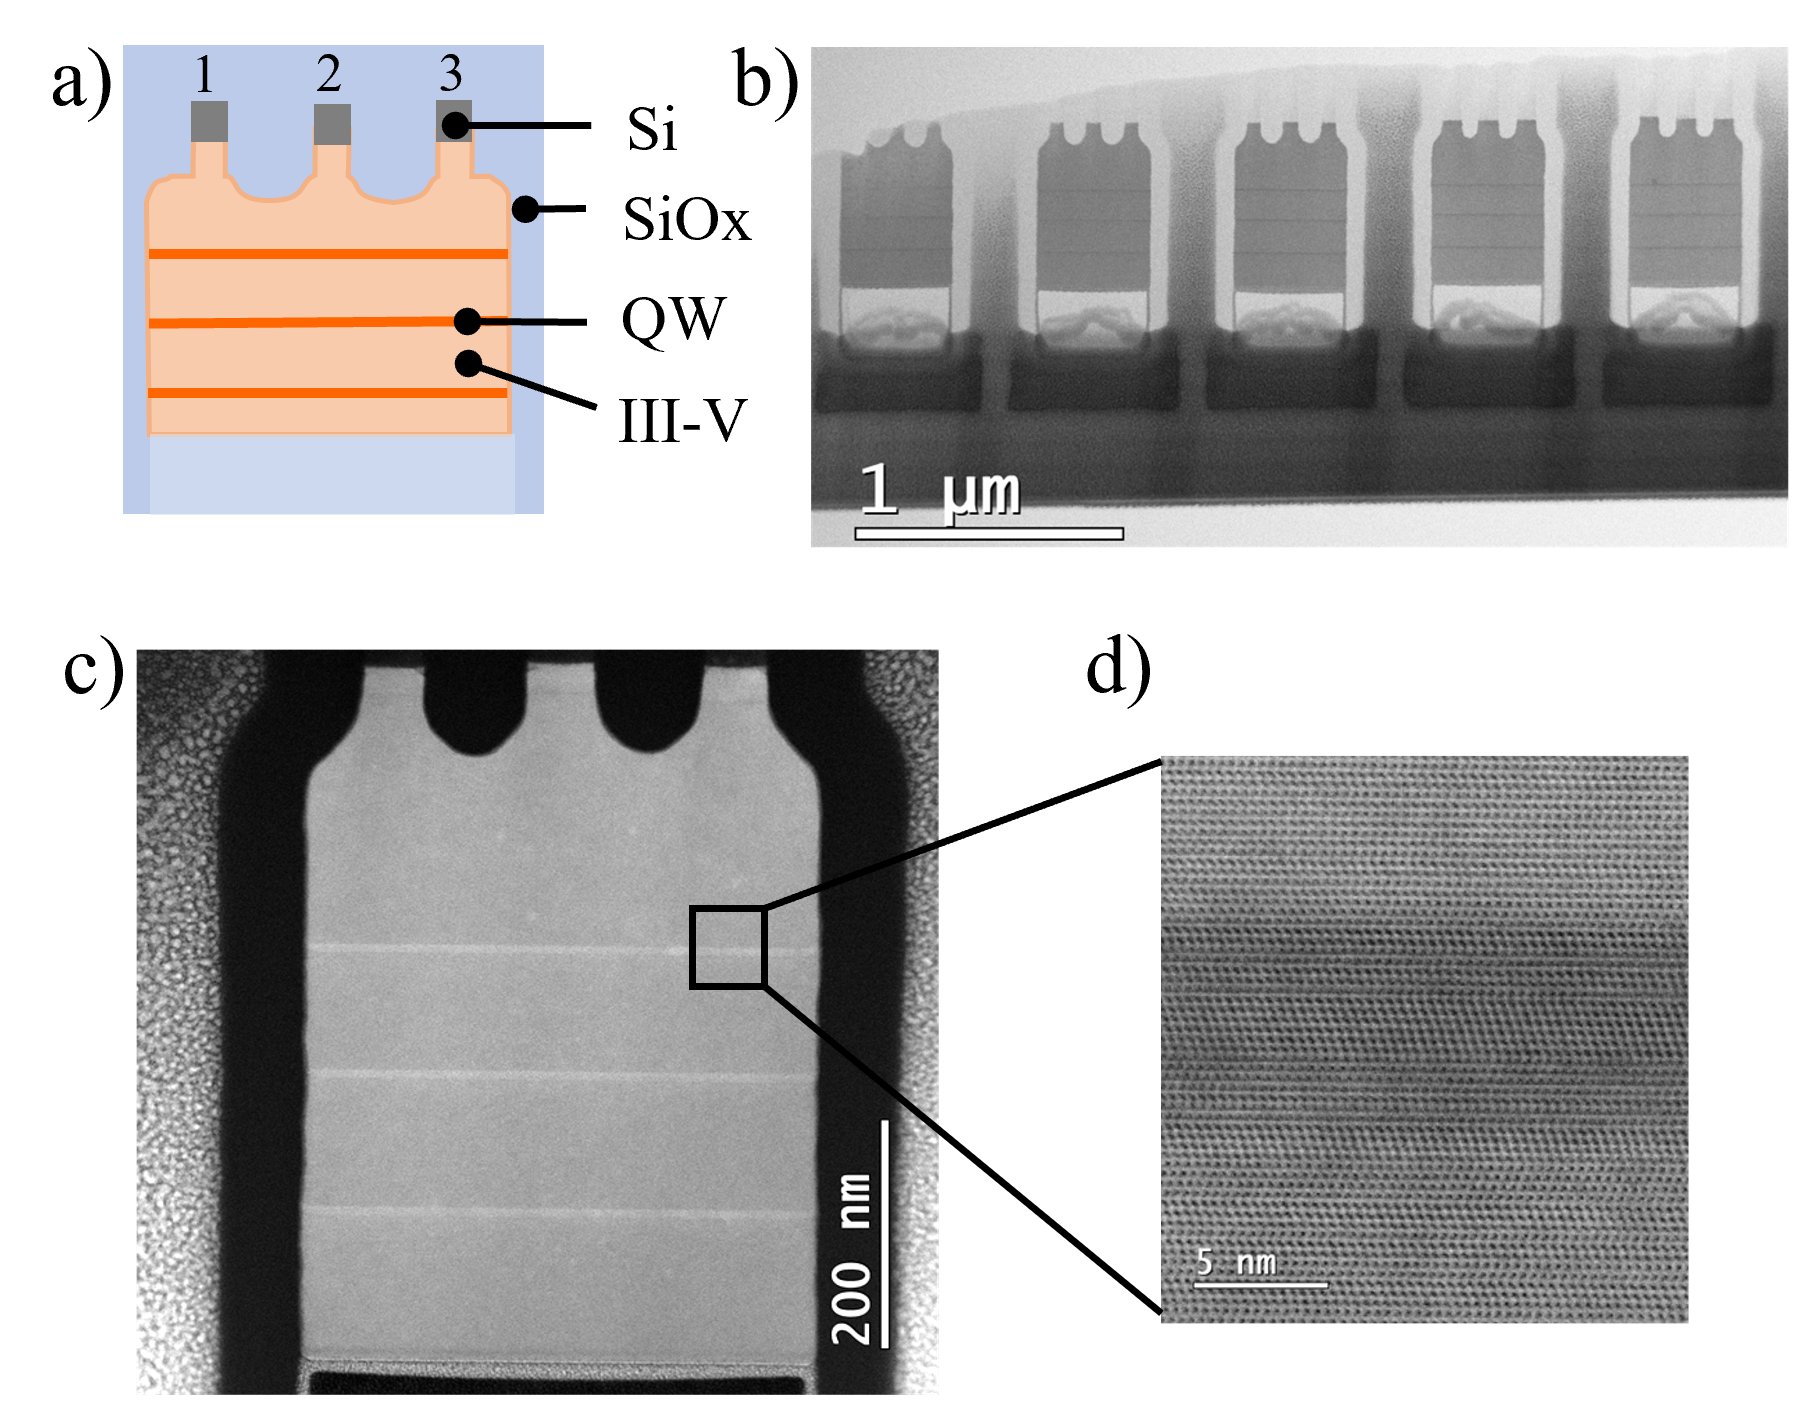
\includegraphics{4_Crystalline_properties/From_Article2/Figure6.png}
    \caption{STEM analysis of quantum wells created in wide structures from the multiple nucleation sites. (a) Top-view schematic of the structure. b) Plane-view image showing five adjacent structures (c) ADF-STEM image of one structure. (d) High-resolution BF-STEM image of a single quantum well.}
    \label{fig:plane_view}
\end{figure}

To demonstrate the robustness of the developed epitaxy process as well as growth recipes, we fabricated test structures of larger width. Furthermore, the template contains not only one \acs{si} nucleation area, but three. Thus the III-V crystal is nucleated in three points simultaneously and develops into short nanowires. These nanowires are then forced to merge into one large platelet of well-defined geometry. The schematic of the structure is illustrated in Figure~\ref{fig:plane_view}.a.
\par
Figure~\ref{fig:plane_view}.b shows a BF-STEM plane-view image of five adjacent structures after STEM lamella preparation. The image shows a high consistency in the overall size of the grown structures and in the presence of the overall \num{15} quantum wells. A single structure is shown in Figure~\ref{fig:plane_view}.c using annular dark field (ADF-)STEM. The three light grey lines correspond to the \acs{ingaas} quantum wells. The high-resolution BF-STEM image in Figure~\ref{fig:plane_view}.d shows one of these quantum wells appearing in darker grey, with additional contrast from alternating stacking sequences forming twin planes which are commonly observed for \hkl<111>\(_B\) growth\cite{Johansson2006}. The quantum well runs uniformly throughout the entire width of the structure, indicating that the growth at this position took place on a single \hkl{111} plane. No other crystal defects were detected in STEM mode. To increase the sensitivity to detect structural defects, standard TEM analysis was performed as well (Figure~\ref{fig:TEM}).

\begin{figure}
    \centering
    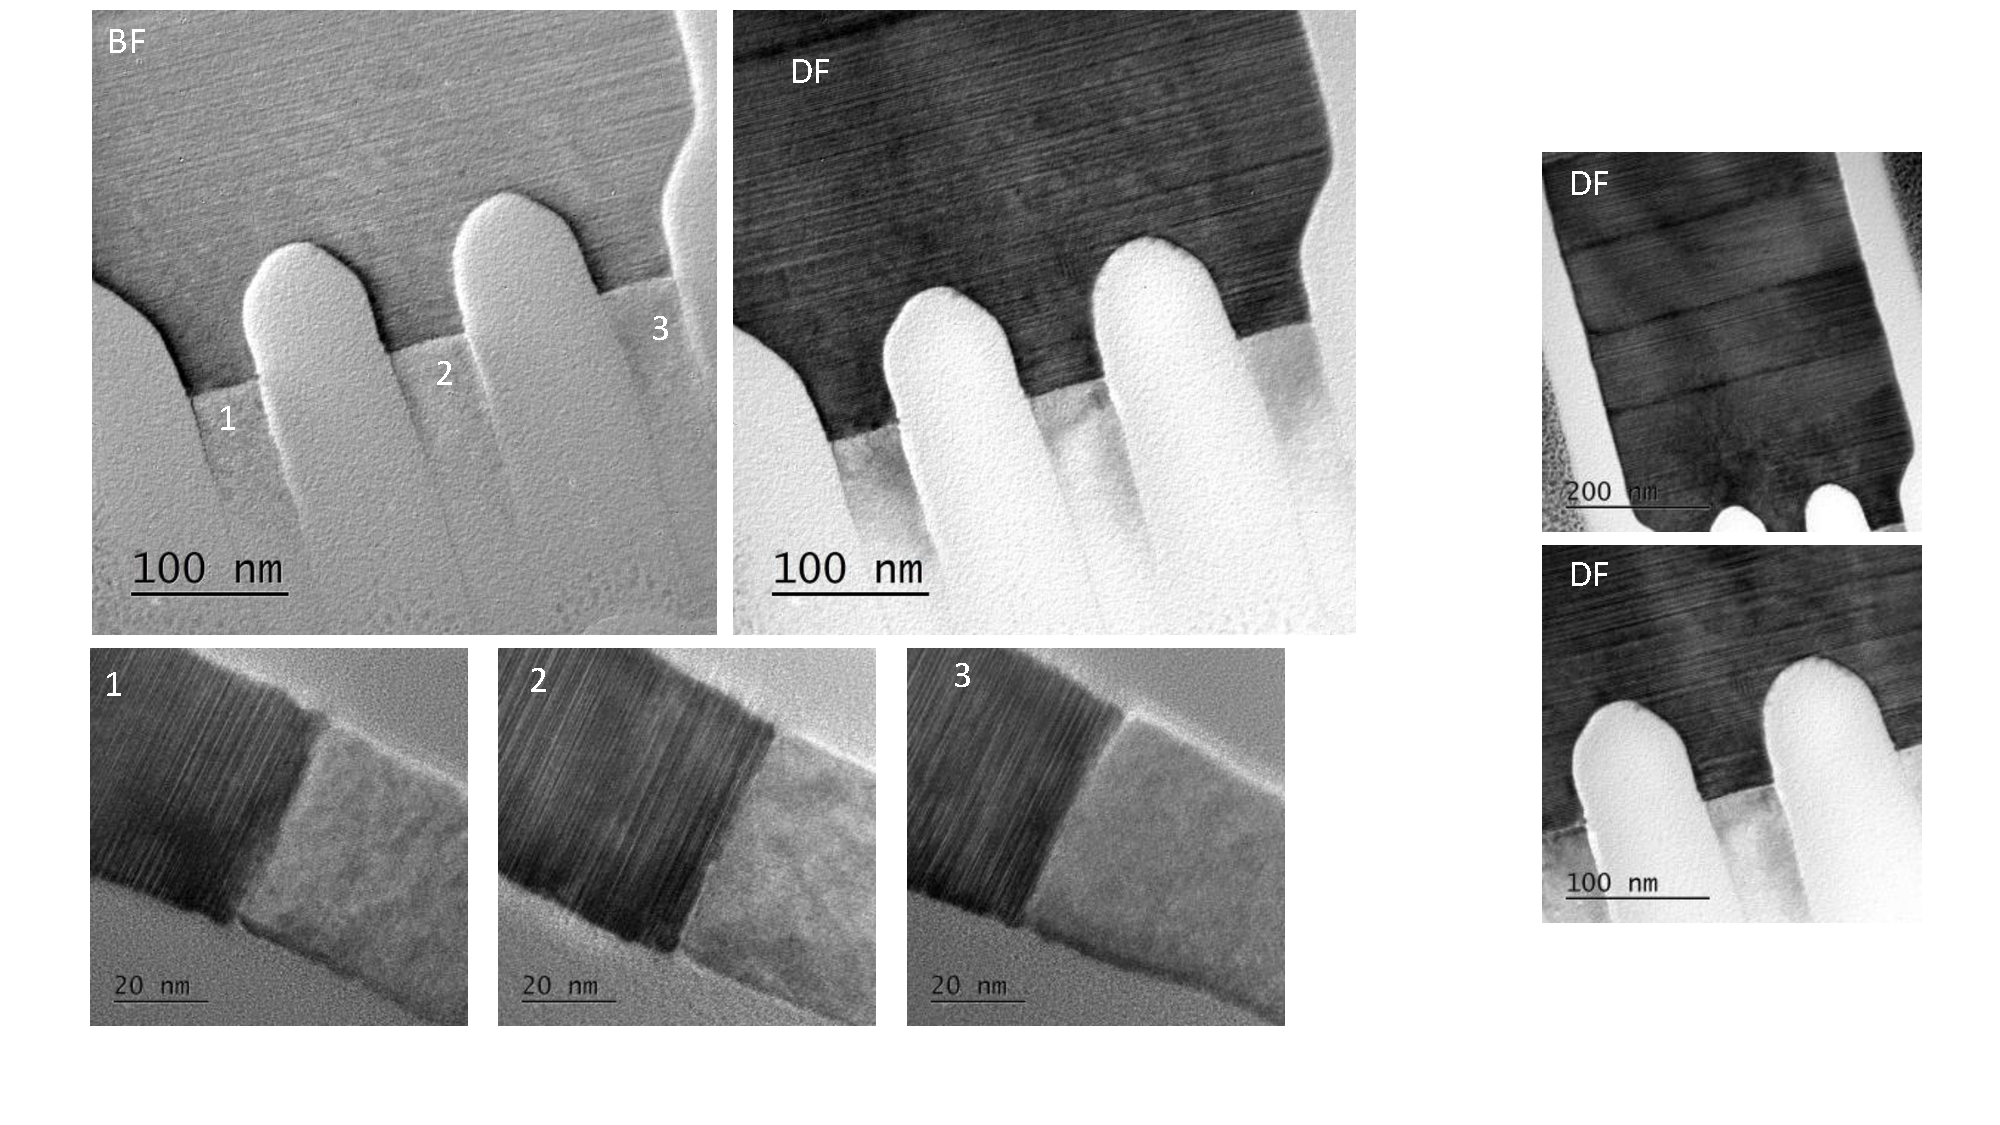
\includegraphics[width = \textwidth]{4_Crystalline_properties/From_Article2/merging_analysis.pdf}
    \caption{TEM analysis of the sampvisualisedFINITIVE FIGURE. PLEASE HEINZ, SEND RAW TEM IMAGES)}
    \label{fig:TEM}
\end{figure}

No propagating dislocations or anti-boundary defects from merging the three initial crystals could be detected. However, this does not exclude the presence of lattice defects which could not be visualised under these imaging conditions. It is unlikely for the three crystal lattices to merge in a perfect registry without the formation of defects\cite{Jacobsson2015, Rossi2023}. However, here the resulting defects remain confined: growth of smooth quantum wells that extend straight across the entire width of the structure would otherwise be impossible.
\par
These observations can be explained by the specific sample geometry, growth directions, and material properties involved. The experiment is arranged in such a way that a \hkl{111} growth front dominates, and no other growth planes are formed. This is achieved by setting a growth condition favouring slow growth along the main \hkl<111> direction and fast growth in the \hkl<110> directions. Under these conditions, efficient step flow occurs on the \hkl{111} facets. In such a configuration, the first wire to extend into the widening template section would spill over the spacre-stabilisesg it from the neighbouring wires and find itself supported on the other wire's \hkl{111} surface. Due to the efficient step flow on the \hkl{111} facets, mismatches of a few monolayers among the three wires are quickly resolved by the formation of one large growth surface that re-stabilises a single \hkl{111} growth front. A single crystal is established beyond these merging points, and growth can extend further into the template cavity.
\par
These structures share strong indications of local growth rate uniformity and simultaneous nucleation. The \num{5.7} width-to-height aspect ratio of the design \qtyproduct{400 x 70}{nm} cross-section is higher than the \num{5} width-to-height aspect ratio (\qtyproduct{3000 x 500}{nm} cross-section) used by \citeauthor{Han2020} and shows a marked improvement in the control of shape and thickness of internal heterostructures. Further, our growth (carried out at \qty{580}{\degreeCelsius}) results are consistent with those obtained homoepitaxially at \qty{570}{\degreeCelsius} with a width-to-height cross-section of \num{20} by \citeauthor{Goswami2020}.